\documentclass[12pt,twoside]{article}

\input{macros-sp26}
\newcommand{\thelecturenum}{10}

\title{CS336 Lecture 10}

\begin{document}

\handout{Lecture \thelecturenum: Efficient Inference}

\setlength{\parindent}{0pt}

\subsection*{Landscaping the Inference Wordload}

Inference shows up in many places:
\begin{itemize}
    \item Actual use (chatbots, code completion, agents, batch data processing)
    \item Model evaluation (e.g., on instruction following)
    \item Reinforcement learning (sample many generations, then apply score)
\end{itemize}

Why \textbf{efficiency} matters: training is one-time cost, inference is repeated many times
\begin{itemize}
    \item OpenAI processes ~8.6T tokens per day
    \item For reference, DeepSeek v4 was trained on 32T tokens
\end{itemize}

Moreover:
\begin{itemize}
    \item Chatbots: most tokens are meant for human consumption (humans are bottleneck)
    \item Agents: query \(\to\) internal trace \(\to\) output for human (number of tokens generated can grow unbounded)
    \item Tokens generated = compute spent
\end{itemize}

Companies doing inference (a big deal for anyone who has a product or platform):
\begin{itemize}
    \item Providers serving closed models (OpenAI, Anthropic, Google, etc.)
    \item Providers serving open-weight models (Together, Fireworks, Baseten, DeepInfra, Groq, Cerebras, etc.)
\end{itemize}

Open-source packages:
\begin{itemize}
    \item vLLM: from Berkeley, pioneered PagedAttention, popular and good default
    \item SGLang: from Berkeley, pioneered RadixAttention, good for agentic workloads
    \item TensorRT-LLM: from NVIDIA, highly optimized for GPUs
    \item llama.cpp: C++ only, supports CPU inference, runs locally
\end{itemize}

\begin{center}
    \textbf{Inference is huge. Important to make it fast.}
\end{center}

What does "fast" mean (metrics)?
\begin{itemize}
    \item Time-to-first-token (TTFT): how long user waits before any generation happens (for interactive applications)
    \item Latency (seconds/token): how fast tokens appear for one query (for interactive applications)
    \item Throughput (tokens/second): how fast tokens appear for many queries (for batch processing)
\end{itemize}

What governs efficiency?
\begin{itemize}
    \item Training (supervised): you see all tokens, can parallelize over sequence (matmul in Transformer)
    \item Inference: you have to generate sequentially, can't parallelize over generation, so harder to fully utilize compute
\end{itemize}

\subsubsection*{Review of Transformers}

\begin{figure}[hpbt]
    \centering
    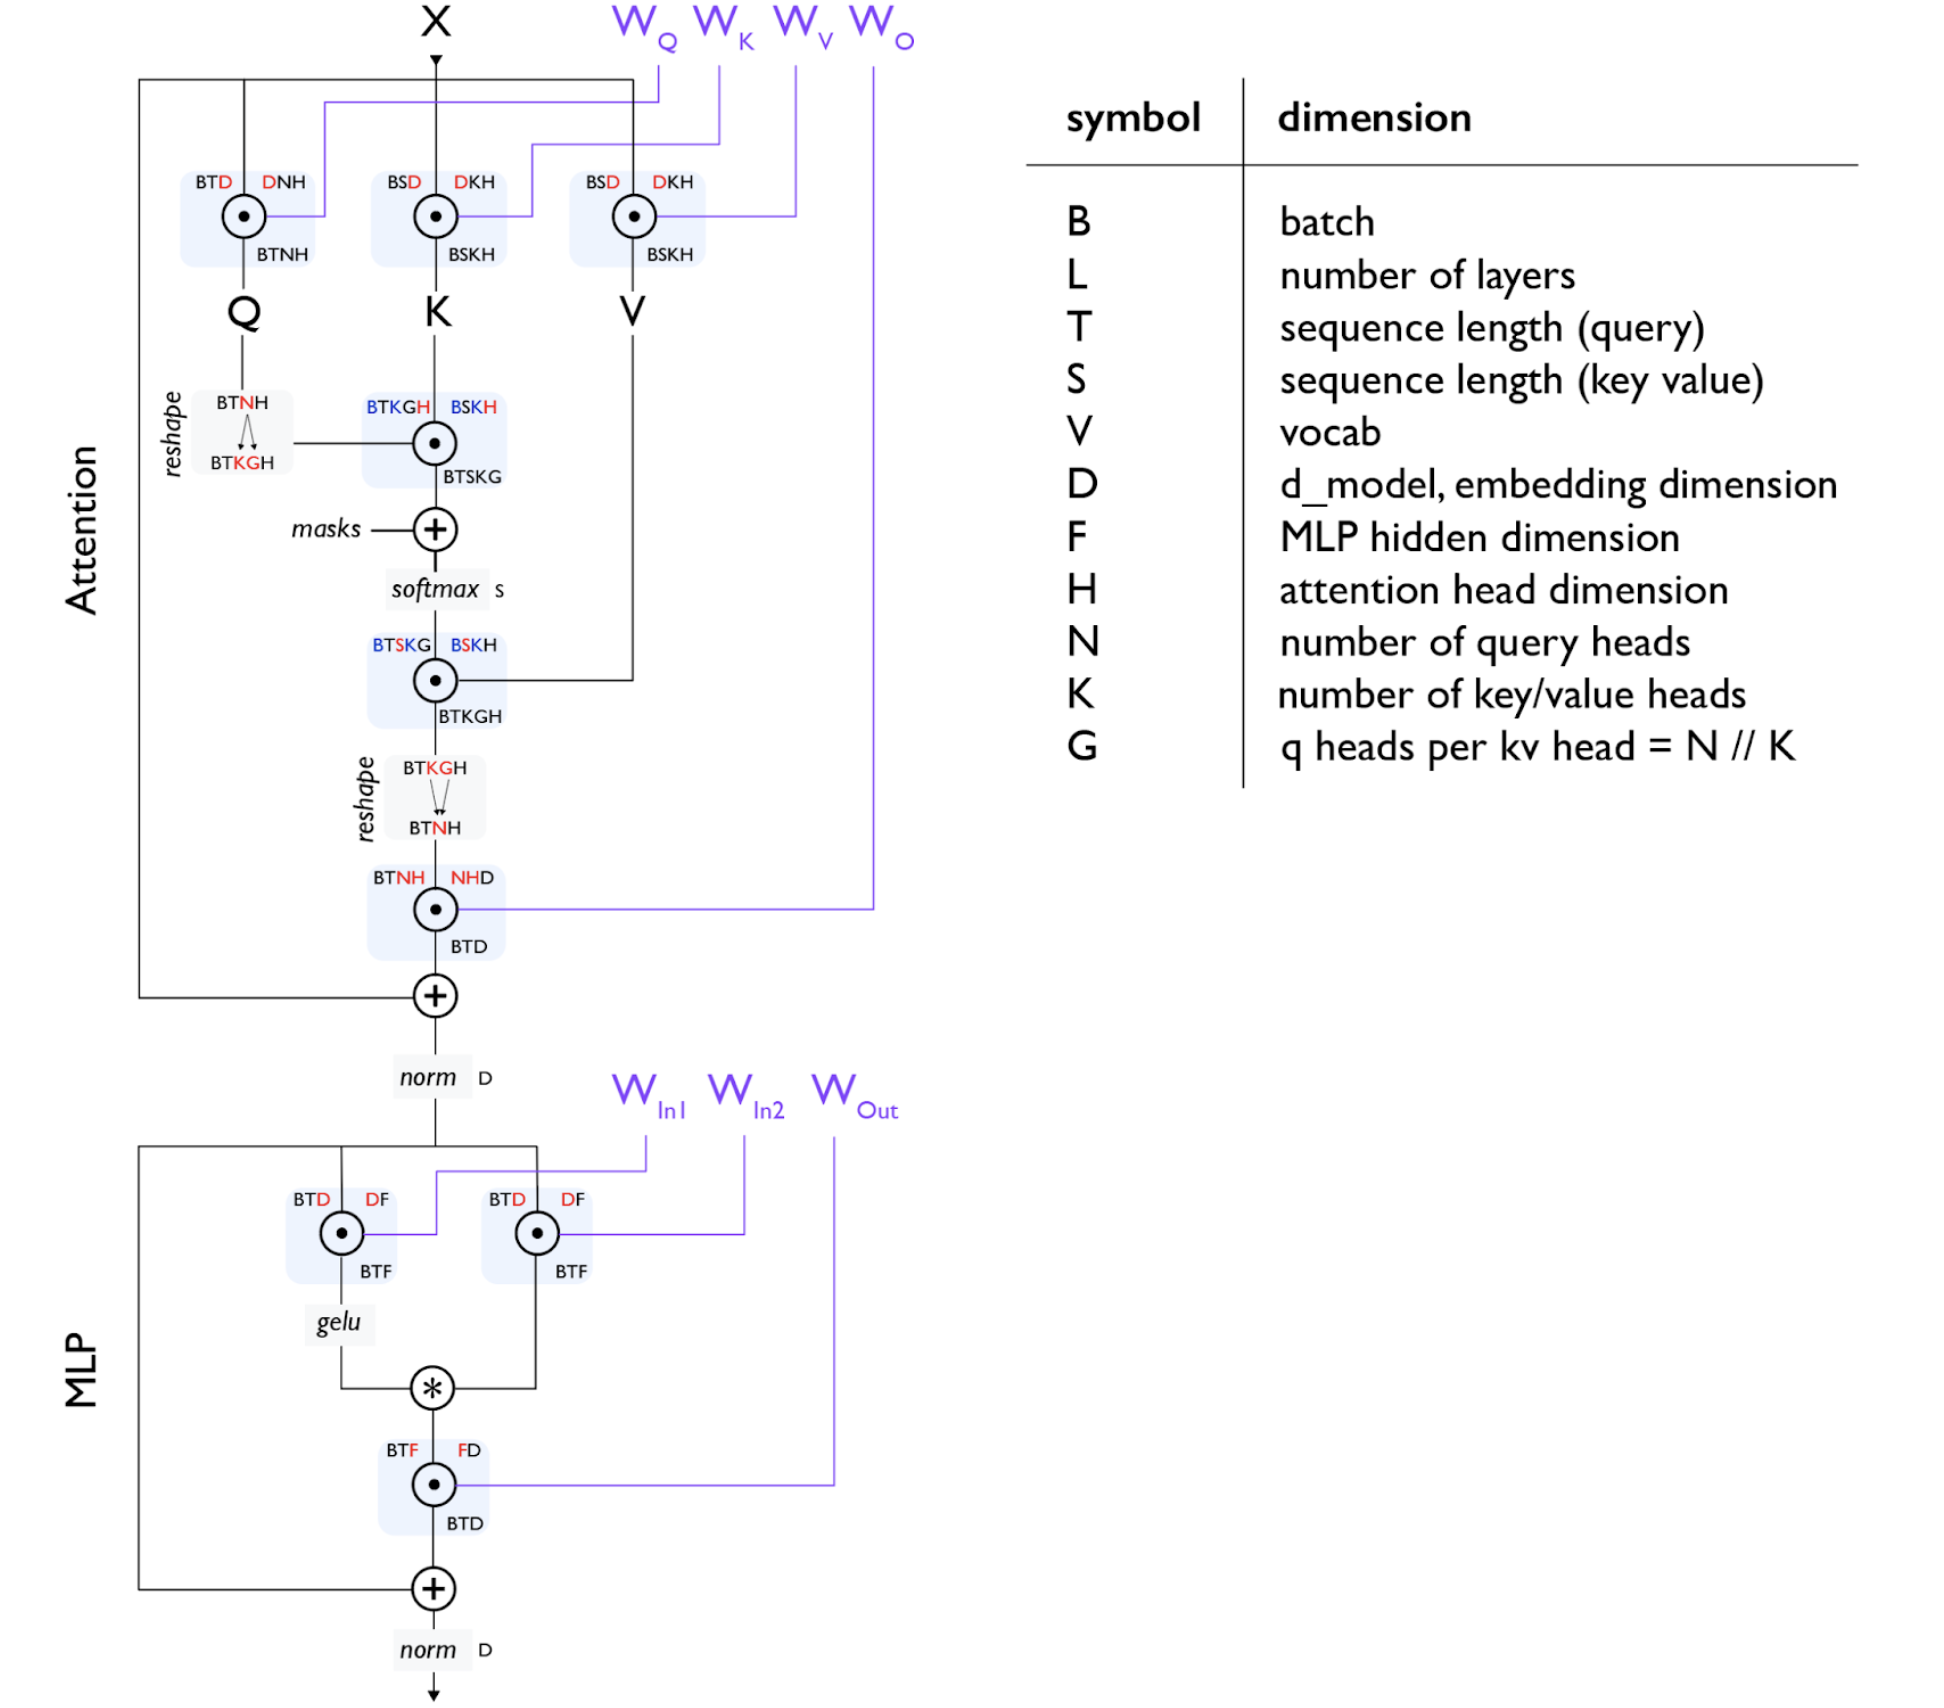
\includegraphics[width=0.92\linewidth]{transform.png}
\end{figure}

Notation (similar to einops):
\begin{itemize}
    \item Symbols denote dimensions (and their length): B (batch), T (sequence), D (model dim), H (head dim)
    \item Example: BTD \(\times\) DH \(\to\) BTH
    \item Contracting dimensions appear in both operands and disappear from result
    \item Regular dimensions appear in one operand and stay in result
    \item Example: BD \(\times\) BD \(\to\) B
    \item Batching dimensions appear in both operands and stay in result
\end{itemize}

Conventions:
\begin{itemize}
    \item F \(=\) 4 D (MLP up-projects into 4\(\times\) the model dimension)
    \item D \(=\) N H (model dimension split across N heads)
    \item N \(=\) K G (for GQA, number of heads split across K groups)
    \item S \(=\) T (during training, condition on S input tokens to predict T output tokens)
\end{itemize}

\subsubsection*{Review of Arithmetic Intensity}

\begin{enumerate}
    \item Setup: multiply X (B x D) and W (D x F) matrix!
    \item Intuition: B is batch size, D is hidden dimension, F is up-projection dimension in MLP.
\end{enumerate}

Let's do FLOPs and memory read/write accounting for the matrix multiplication (X \(*\) W).

\begin{minted}{python}
    flops = 0
    bytes_transfered = 0
    
    # Perform the operation
    1. Read X (B \(\times\) D) from HBM
    bytes_transferred += 2*B*D   # 2 bytes for bf16
    2. Read W (D \(\times\) F) from HBM
    bytes_transferred += 2*D*F
    3. Compute Y \(=\) X (B \(\times\) D) @ W (D \(\times\) F)
    flops += 2*B*D*F
    4. Write Y (B \(\times\) F) to HBM
    bytes_transferred += 2*B*F
    
    assert flops == 2*B*D*F
    assert bytes_transferred == 2*B*D + 2*D*F + 2*B*F
\end{minted}

Recall that \textbf{arithmetic intensity} is how much compute we do per byte transferred (want to be high).

\begin{minted}{python}
    intensity = (flops / bytes_transferred).simplify()
\end{minted}

Assuming B is much less than D and F, then we can simplify:

\begin{minted}{python}
    intensity.subs(D, c*B).subs(F, c*B).limit(c, oo).simplify()  
    assert intensity == B
\end{minted}

Accelerator intensity of H100:

\begin{minted}{python}
    flops_per_second = 989e12
    memory_bandwidth = 3.35e12
    accelerator_intensity = flops_per_second / memory_bandwidth 
    assert round(accelerator_intensity) == 295
\end{minted}

\begin{center}
    Conclusion: compute-bound iff B \(>\) 295.
\end{center}

Extreme case (B \(=\) 1, corresponding to matrix-vector product):
\begin{itemize}
    \item Arithmetic intensity: 1
    \item Memory-bound (read D \(\times\) F matrix, perform only 2 D F FLOPs)
    \item This is basically what happens with inference...
\end{itemize}

\subsection*{Arithmetic Intensity of Inference}

\begin{figure}[hpbt]
    \centering
    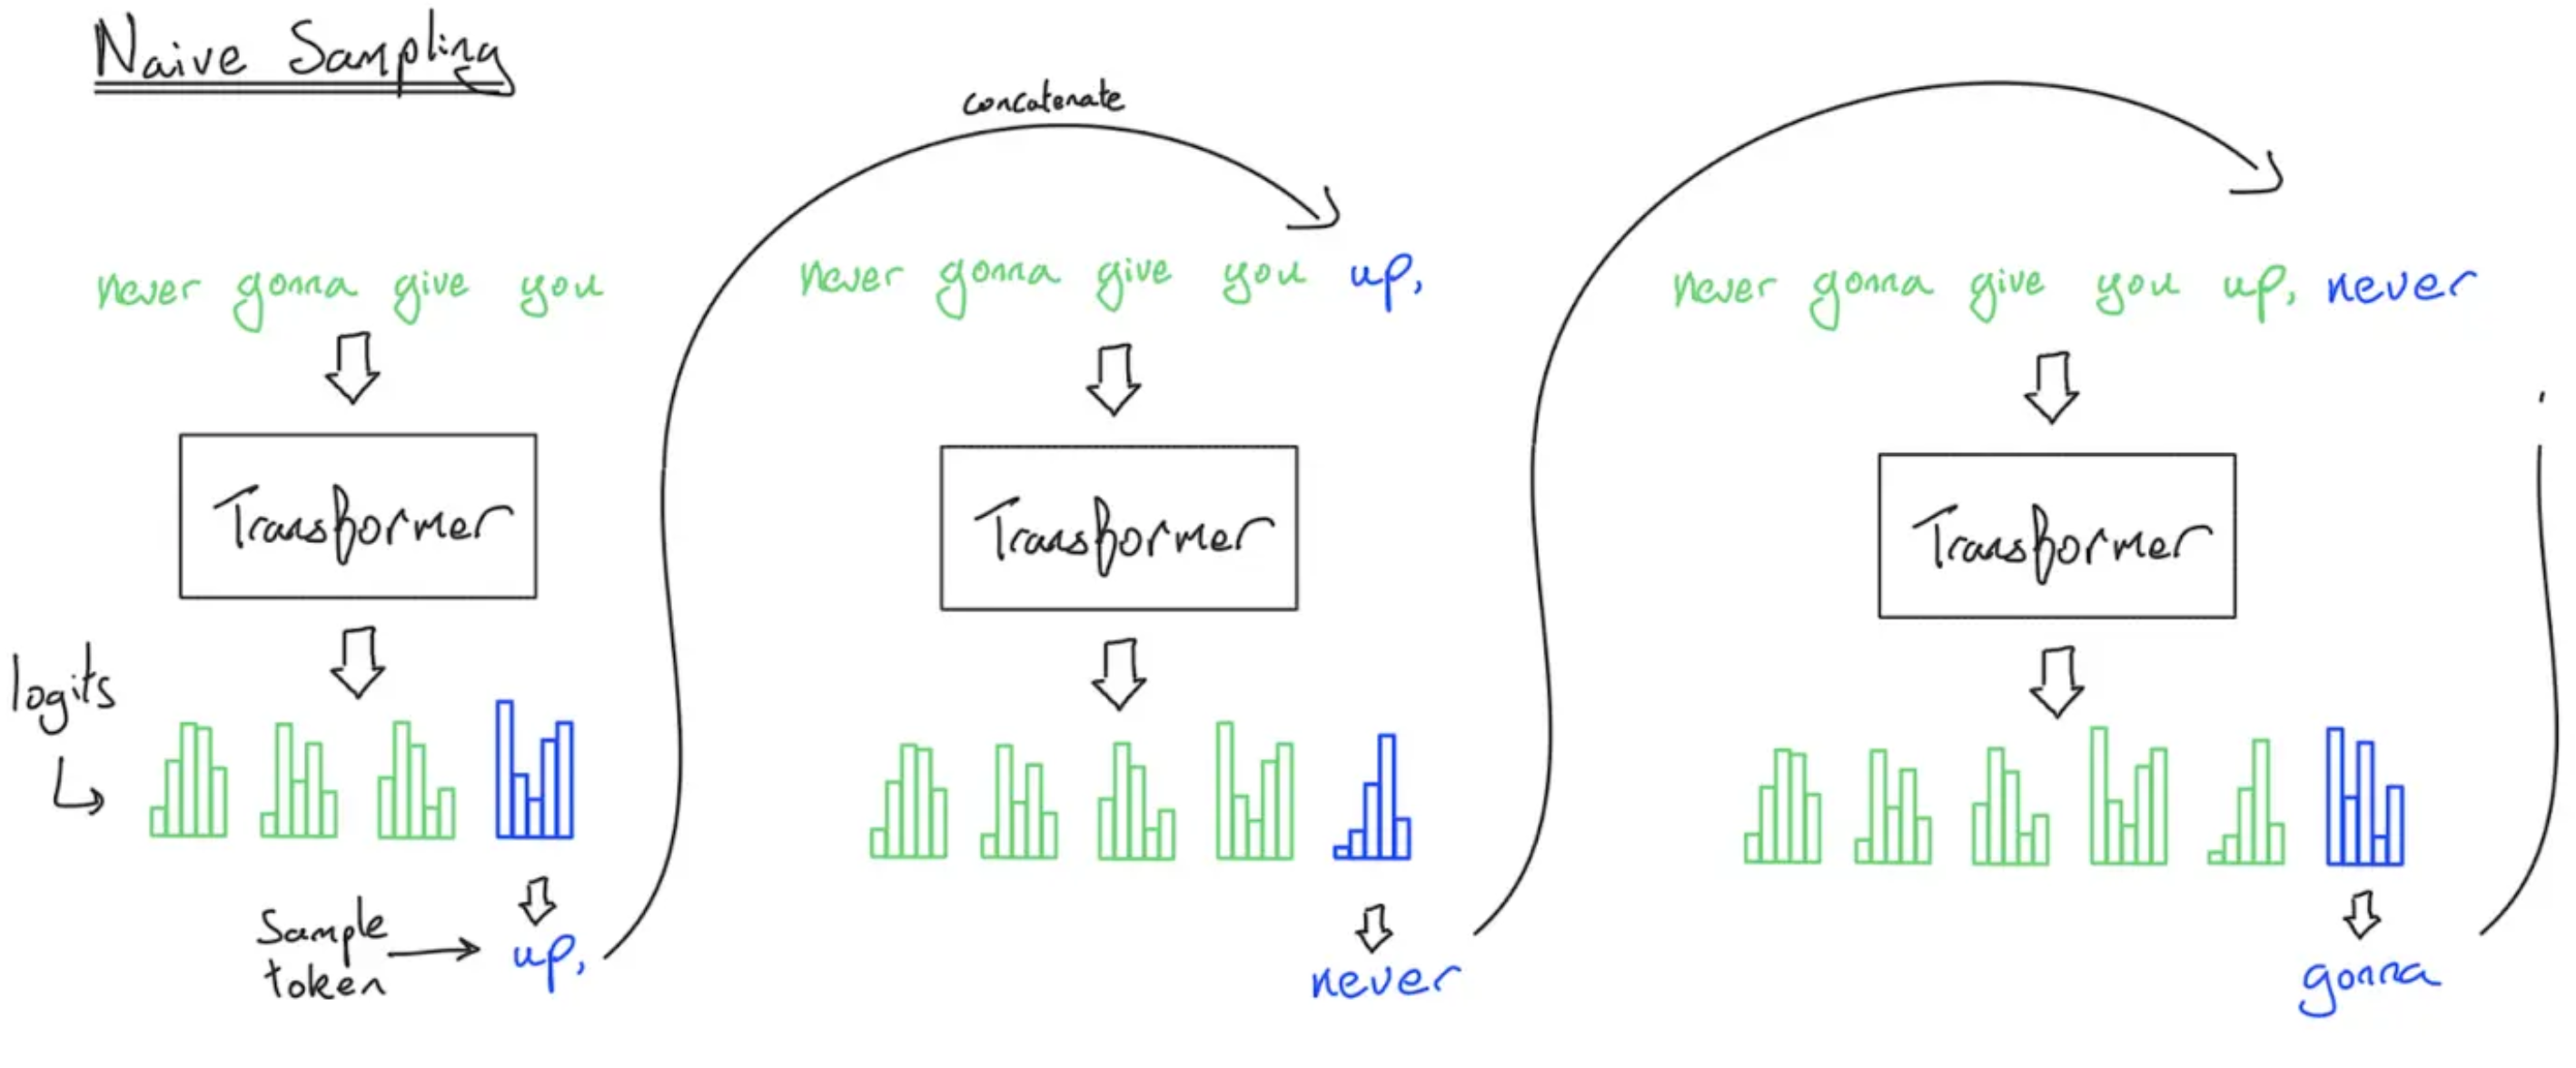
\includegraphics[width=1\linewidth]{naive_decoding.png}
\end{figure}

\begin{enumerate}
    \item Naive inference: to generate each token, feed history into Transformer
    \item Complexity: generating T tokens requires \(O(T^3)\) FLOPs (one feedforward pass is \(O(T^2))\)
    \item Observation: a lot of the work can be shared across prefixes
    \item Solution: store KV cache in HBM
\end{enumerate}

\begin{figure}[hpbt]
    \centering
    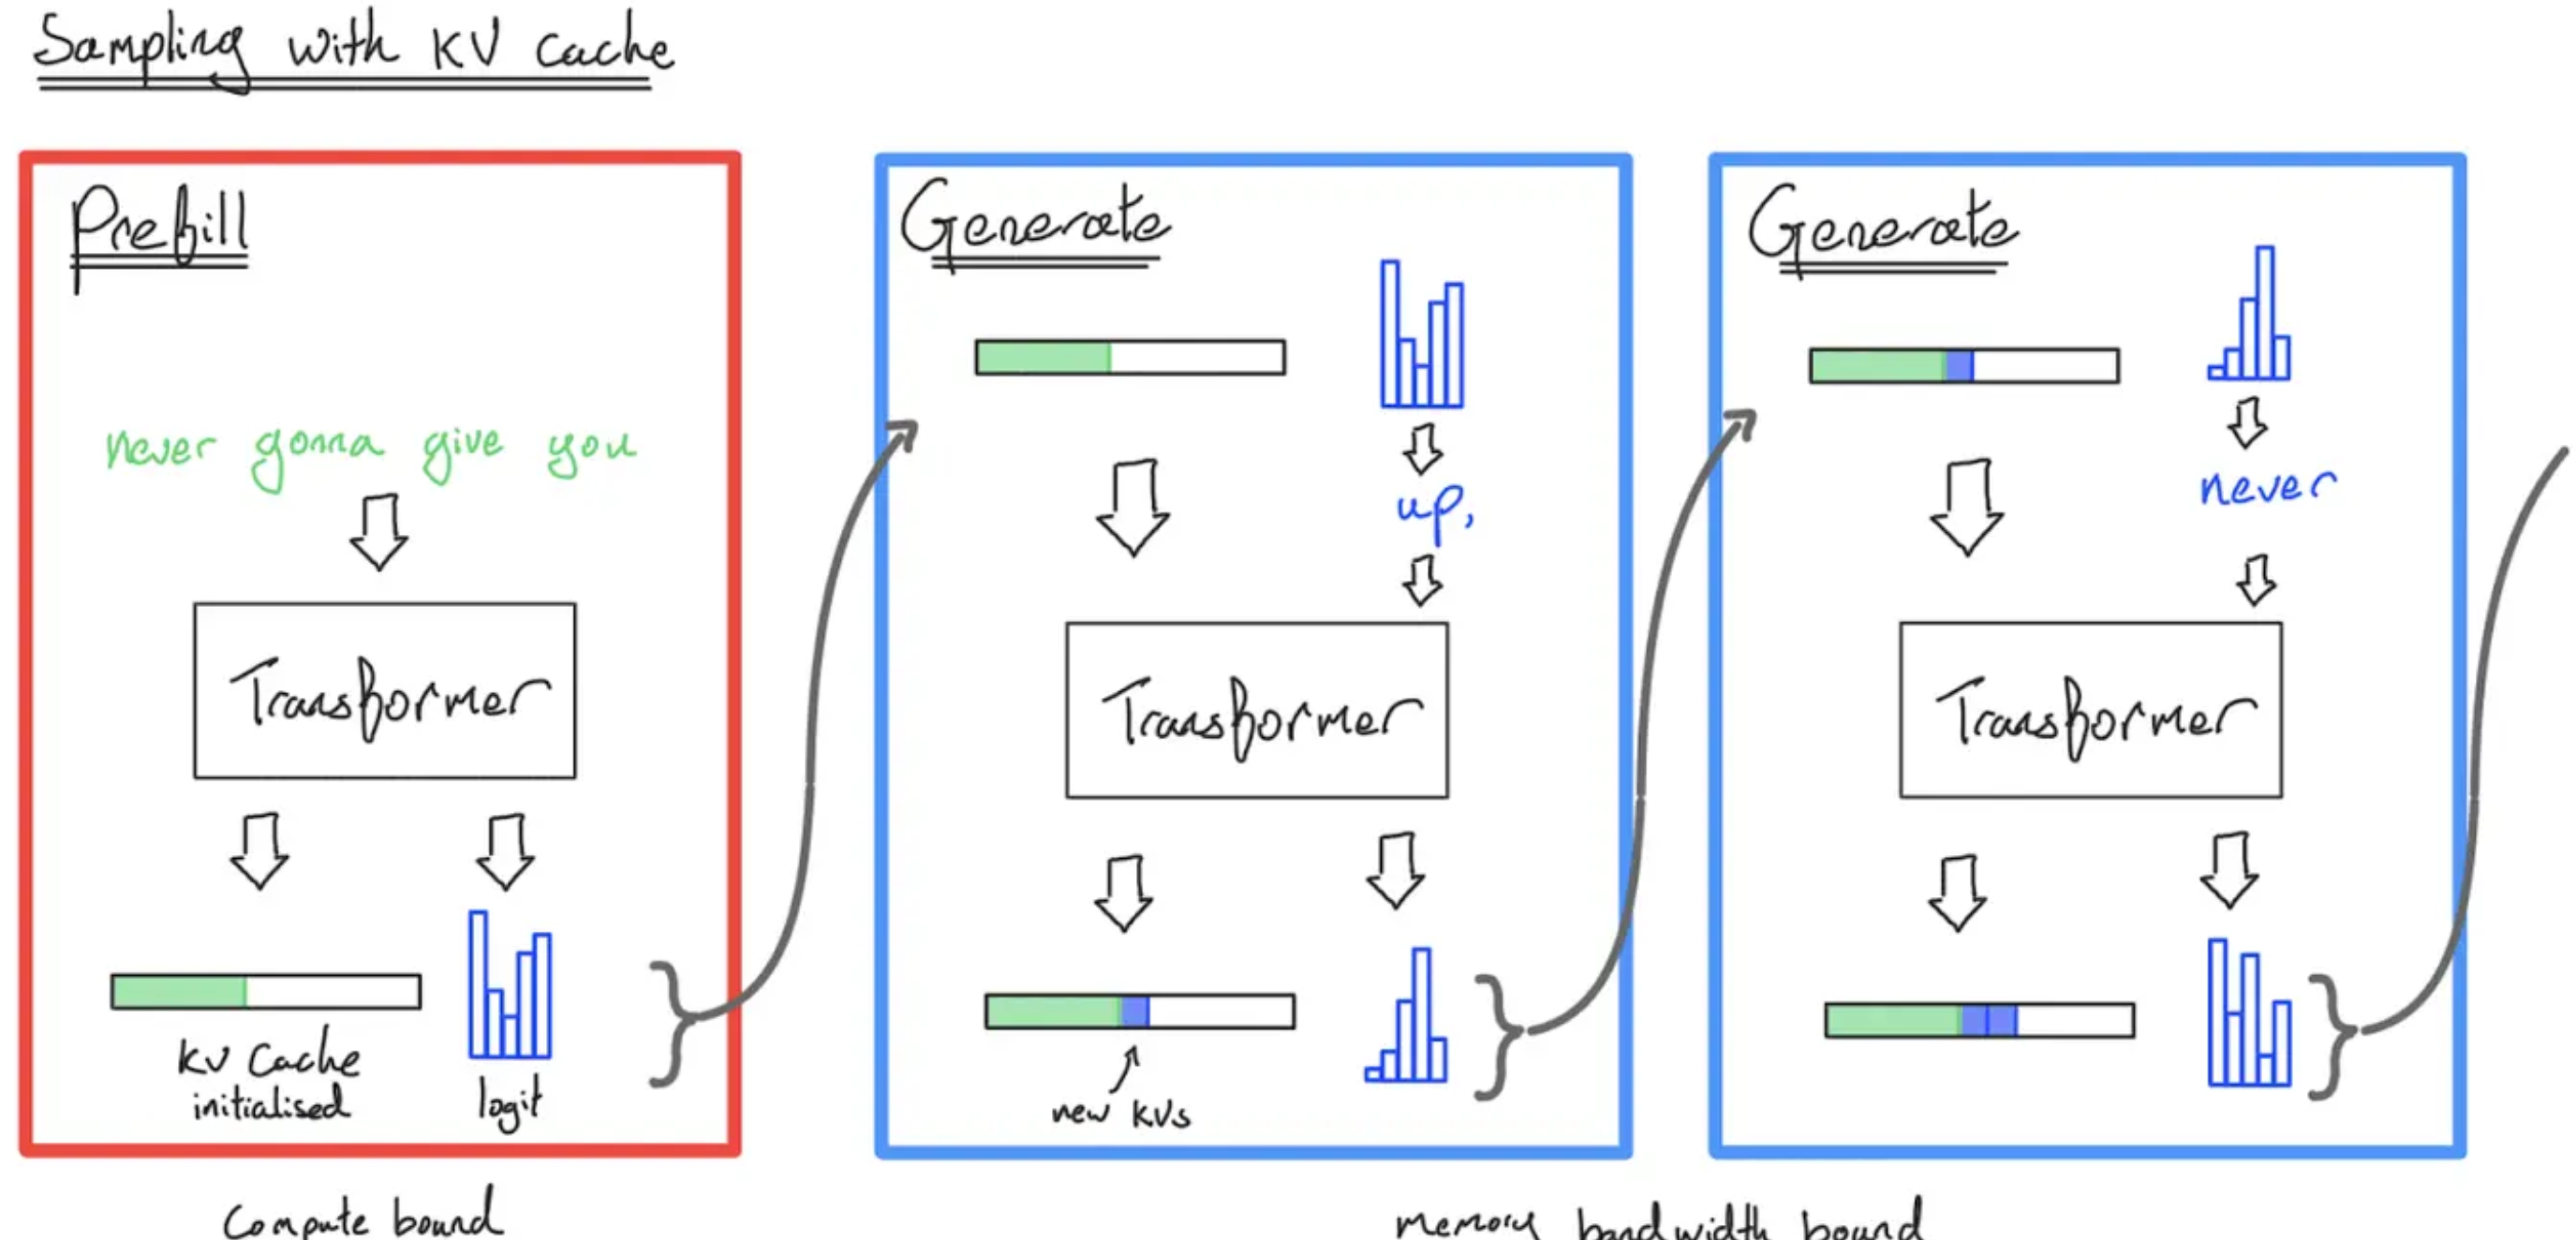
\includegraphics[width=1\linewidth]{kv_caching.png}
\end{figure}

\begin{center}
    KV cache: for every sequence (B), token (S), layer (L), head (K), store an H-dimensional vector
\end{center}

Tow stages of inference:
\begin{enumerate}
    \item \textbf{Prefill}: given a prompt, encode into vectors (parallelizable like in training)
    \item \textbf{Generation}: generate new response tokens (sequential)
\end{enumerate}

Let's compute the FLOPs and memory IO for both the MLP and attention layers.

\begin{itemize}
    \item S is the number of tokens we're conditioning on, T is the number of tokens we're generating.
    \item Later, we'll specialize to prefill (T = S) and generation (T = 1).
\end{itemize}

\subsubsection*{MLP layers (only looking at the matrix multiplication}

\begin{minted}{python}
    flops = 0
    bytes_transferred = 0
    
    # Perform the operation
    1. Read X (B x T x D) from HBM
    bytes_transferred += 2*B*T*D
    2. Read Wup (D x F), Wgate (D x F), Wdown (F x D) from HBM
    bytes_transferred += 3 * 2*D*F
    3. Compute U = X (B x T x D) @ Wup (D x F)
    flops += 2*B*T*D*F
    4. Write U (B x T x F) to HBM
    bytes_transferred += 2*B*T*F
    5. Compute G = X (B x T x D) @ Wgate (D x F)
    flops += 2*B*T*D*F
    6. Write G (B x T x F) to HBM
    bytes_transferred += 2*B*T*F
    7. Compute Y = GeLU(G)*U (B x T x F) @ Wdown (F x D)
    flops += 2*B*T*D*F
    8. Write Y (B x T x D) to HBM
    bytes_transferred += 2*B*T*D
    
    assert flops == 6*B*T*D*F
    assert bytes_transferred == 4*B*T*D + 4*B*T*F + 6*D*F
    
    # Compute the arithmetic intensity
    intensity = (flops / bytes_transferred).simplify()  
    9. Assume that B*T is much smaller than D and F.
    intensity.subs(D, c*B*T).subs(F, c*B*T).limit(c, oo).simplify()  
    assert intensity == B*T
\end{minted}

For the two stages:
\begin{enumerate}
    \item Prefill: easy to make compute-bound (good) by making B*T large enough (large batches, long sequences)
    \item Generation: two problems
    \begin{itemize}
        \item Generating one token at a time (T \(=\) 1)
        \item B is number of concurrent requests, unpredictable for interactive applications
    \end{itemize}
\end{enumerate}

\subsubsection*{Attention layers (focusing on the matrix multiplications with FlashAttention)}

\begin{itemize}
    \item S is number of previous tokens (already generated)
    \item T is number of next tokens (to generate logits for)
\end{itemize}

\begin{minted}{python}
    flops = 0
    bytes_transferred = 0
    
    # Perform the operation
    1. Read Q (B x T x D), K (B x S x D), V (B x S x D) from HBM
    bytes_transferred += 2*B*T*D + 2*B*S*D + 2*B*S*D
    2. Compute A = Q (B x T x D) @ K (B x S x D)
    flops += 2*B*S*T*D
    3. Compute Y = softmax(A) (B x S x T x K x G) @ V (B x S x K x H)
    flops += 2*B*S*T*D
    4. Write Y (B x T x D) to HBM
    bytes_transferred += 2*B*T*D
    
    assert flops == 4*B*S*T*D
    assert bytes_transferred == 4*B*S*D + 4*B*T*D
    
    # Compute the arithmetic intensity
    intensity = (flops / bytes_transferred).simplify()  
    assert intensity == S*T / (S + T)
\end{minted}

For the two stages:
\begin{enumerate}
    \item Prefill: S \(=\) T
\begin{minted}{python}
prefill_intensity = intensity.subs(T, S).simplify() 
assert prefill_intensity == S/2  # Good!
\end{minted}
    \item Generation: T \(=\) 1
\begin{minted}{python}
generate_intensity = intensity.subs(T, 1).simplify()
assert generate_intensity < 1  # Bad!
\end{minted}
\end{enumerate}

Unlike MLPs, no dependence on B, so batching doesn't help!
\begin{itemize}
    \item In MLP layers, every sequence hits the same MLP weights (Wup, Wgate, Wdown don't depend on B)
    \item In attention layers, every sequence has its own KV cache vectors (Q, K, V all depend on B)
\end{itemize}

Summary:
\begin{itemize}
    \item Prefill is compute-bound, generation is memory-bound
    \item Prefill MLP intensity: B\(*\)S
    \item Prefill attention intensity: S \(/\) 2
    \item Generation MLP intensity: B (requires concurrent requests)
    \item Generation attention intensity: \(<\)1 (impossible to improve)
\end{itemize}

\begin{minted}{python}
@dataclass(frozen=True)
class TransformerPerformanceStats:
    """
    Performance stats of a Transformer:
    - num_params: number of parameters (in bytes)
    - memory: total memory usage (parameters + KV cache) in bytes
    - latency: time to generate one token (seconds/token)
    - throughput: tokens generated per second
    """
    num_params: int
    memory: int
    latency: float
    throughput: float
    
    def substitute(self, key, value):
        """Substitute `key` with `value` in all stats."""
        return TransformerPerformanceStats(
            self.num_params.subs(key, value).simplify(),
            self.memory.subs(key, value).simplify(),
            self.latency.subs(key, value).simplify(),
            self.throughput.subs(key, value).simplify(),
        )

def compute_transformer_performance_stats(
    config) -> TransformerPerformanceStats:  
    """Compute various performance stats for the Transformer"""
    
    # Number of parameters in the Transformer
    num_params = 2*V*D + D*F*3*L + (2*D*N*H + 2*D*K*H)*L
    
    # How much memory the parameters take
    parameter_size = 2*num_params  # 2 for bf16
    
    # How much the KV cache takes per sequence 
    # (S tokens, K heads, H head dim, L layers)
    kv_cache_size_per_seq = S * (K*H) * L * 2 * 2 
    
    # Total memory usage
    memory = B * kv_cache_size_per_seq + parameter_size
    
    # *Latency* is determined by memory IO
    latency = memory / memory_bandwidth
    
    # *Throughput* is the inverse of latency
    throughput = B / latency
    
    # Substitute config
    num_params = num_params.subs(config).simplify()  
    memory = memory.subs(config).simplify()  
    latency = latency.subs(config).simplify()  
    throughput = throughput.subs(config).simplify()  
    
    return TransformerPerformanceStats(
        num_params, memory, latency, throughput)

def llama2_13b_config(args={}):
    return {
        S: 1024,   # Sequence length
        D: 5120,   # Model dim
        F: 13824,  # Feed-forward dim
        N: 40,     # Number of query heads
        K: 40,     # Number of key/value heads
        H: 128,    # Head dimension
        L: 40,     # Number of layers
        V: 32000,  # Vocabulary size
        memory_bandwidth: 3.35e12,  # Memory bandwidth (bytes/second)
        **args
    }
\end{minted}

\subsection*{Throughput and Latency}

Let us now compute the theoretical maximum latency and throughput of a single request.

\begin{center}
    Assumption: can overlap compute and communication perfectly and ignore overhead.
\end{center}

Instantiate latency and throughput for Llama 2 13B on an H100:

\begin{minted}{python}
    config = llama2_13b_config()
    stats = compute_transformer_performance_stats(config)
    
    # Batch size 1
    b1 = stats.substitute(B, 1)  
    
    # Batch size 64
    b64 = stats.substitute(B, 64)  
    Result: worse latency, better throughput
    
    # Batch size 256
    b256 = stats.substitute(B, 256)  
    Result: even worse latency, even better throughput
    h100_memory = 80e9  # H100 memory in bytes
    assert b256.memory > h100_memory  # Doesn't fit in memory!
    Result: doesn't fit into memory and throughput gains are diminishing too...
\end{minted}

What increasing batch size does:
\begin{itemize}
    \item Worsens latency because larger KV cache (\(O(B)\) size) to read/write
    \item Improves throughput because amortizes the cost of reading parameters
\end{itemize}

\textbf{Tradeoff} between latency and throughput:
\begin{itemize}
    \item Smaller batch sizes yield better latency but worse throughput
    \item Larger batch sizes yield better throughput but worse latency
\end{itemize}

\begin{center}
    \textbf{If you launch M copies of the model, latency is the same, throughput increases by M!}    
\end{center}

Note: time-to-first-token (TTFT) is essentially a function of prefill time
\begin{itemize}
    \item Use smaller batch sizes during prefill for faster TTFT
    \item Use larger batch sizes during generation to improve throughput
\end{itemize}

\begin{center}
    \textbf{Shard the model and the KV cache!}
\end{center}

\subsection*{Key-Value Caching}

Recall that memory is the bottleneck for inference. So let's try to reduce the size of the KV cache ... but make sure we don't lose too much accuracy.

\begin{itemize}
    \item Idea: N query heads, but only K key and value heads, each interacting with N / K query heads
    \item Multi-headed attention (MHA): K \(=\) N
    \item Multi-query attention (MQA): K \(=\) 1
    \item Group-query attention (GQA): K is somewhere in between
\end{itemize}

Latency/throughput improves: 

\begin{figure}[H]
    \centering
    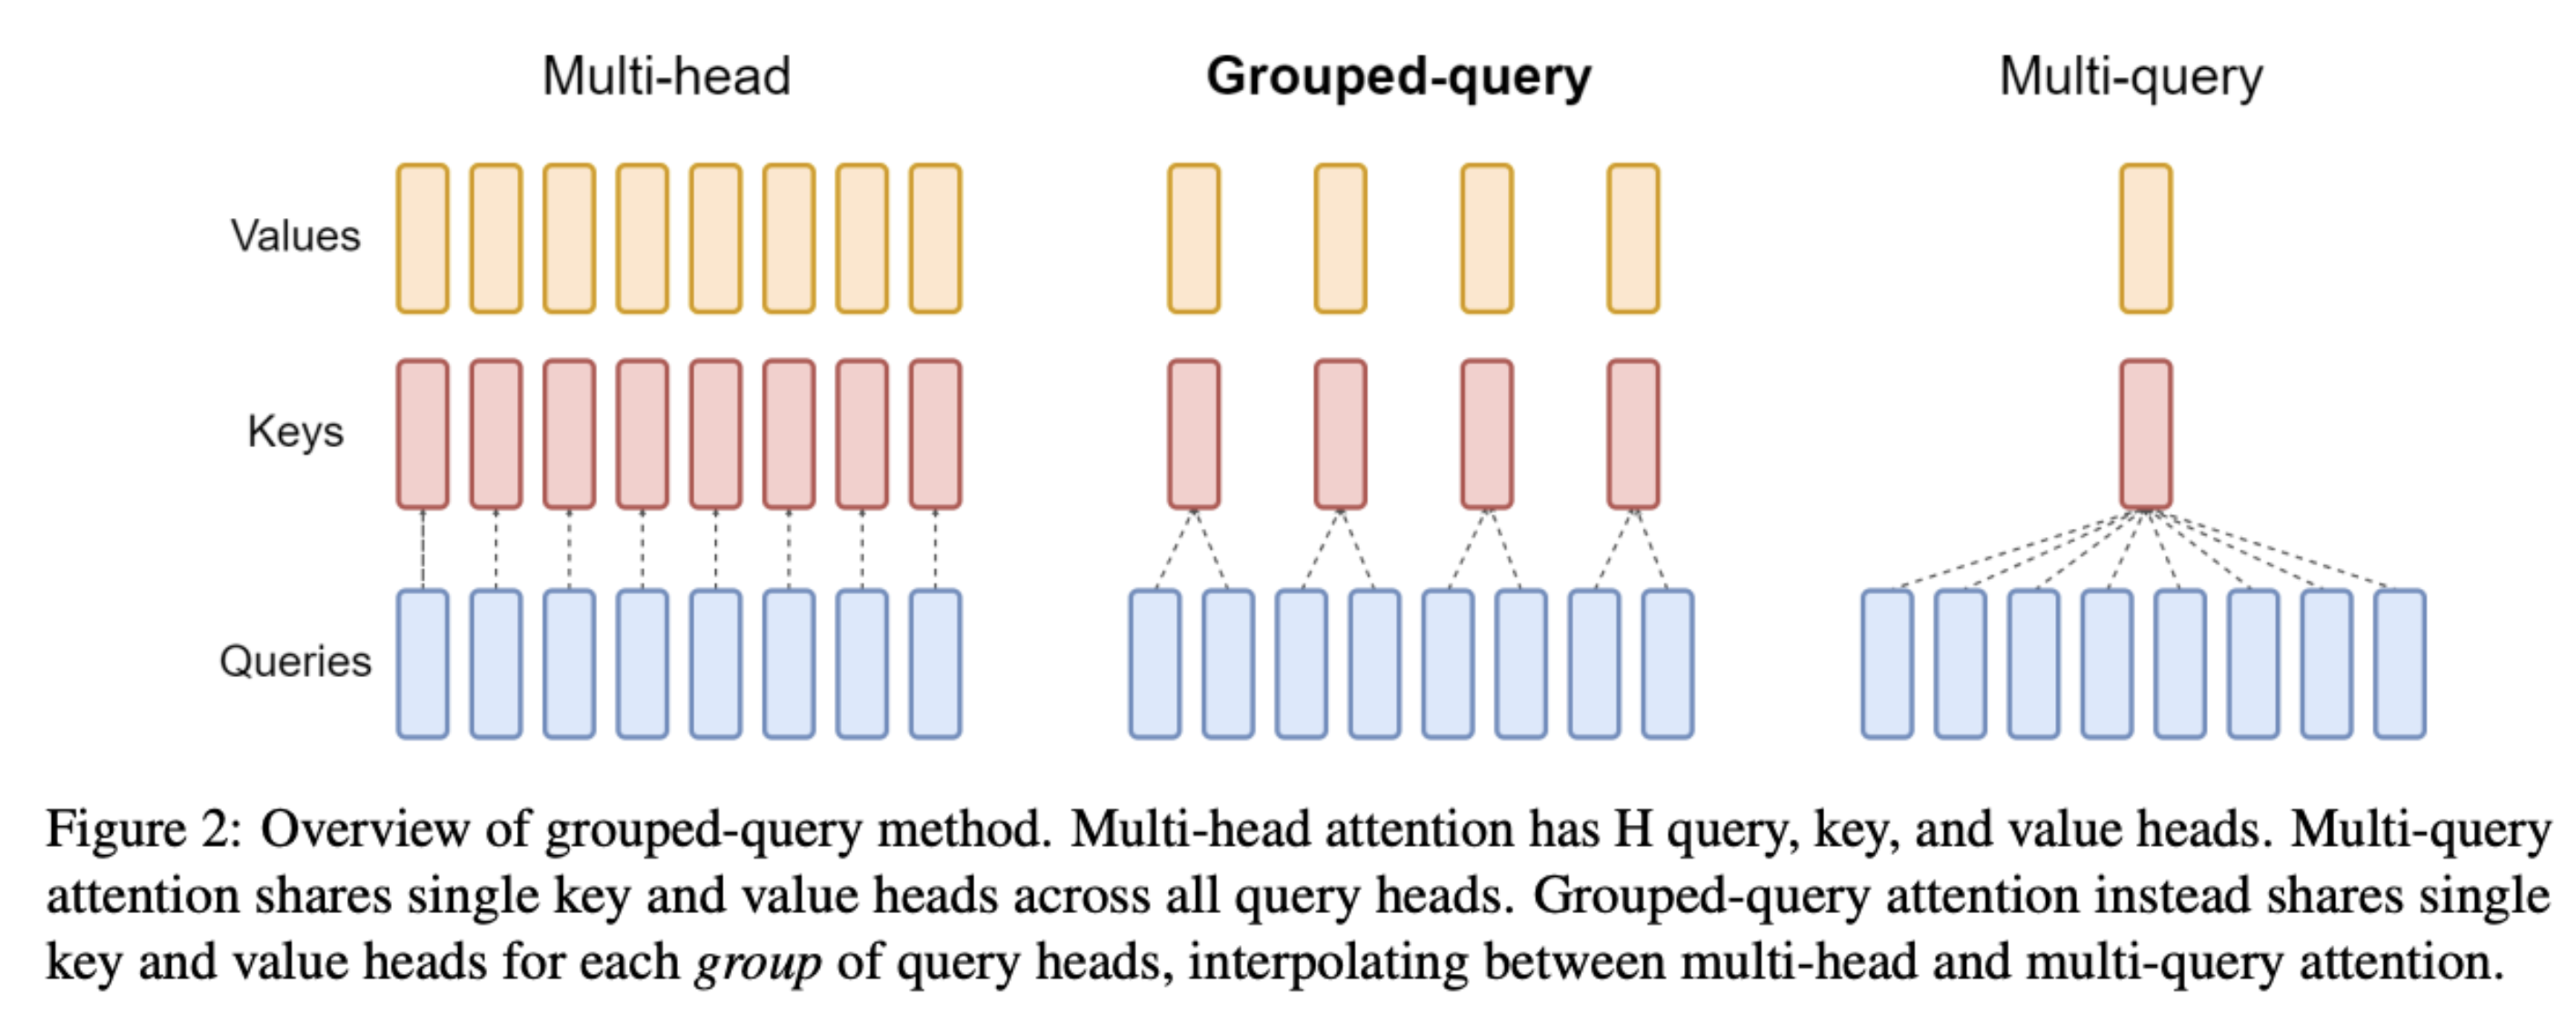
\includegraphics[width=1\linewidth]{GQA.png}
\end{figure}

\begin{question}
    Why does GQA improve latency and throughput?
\end{question}

\begin{figure}[hpbt]
    \centering
    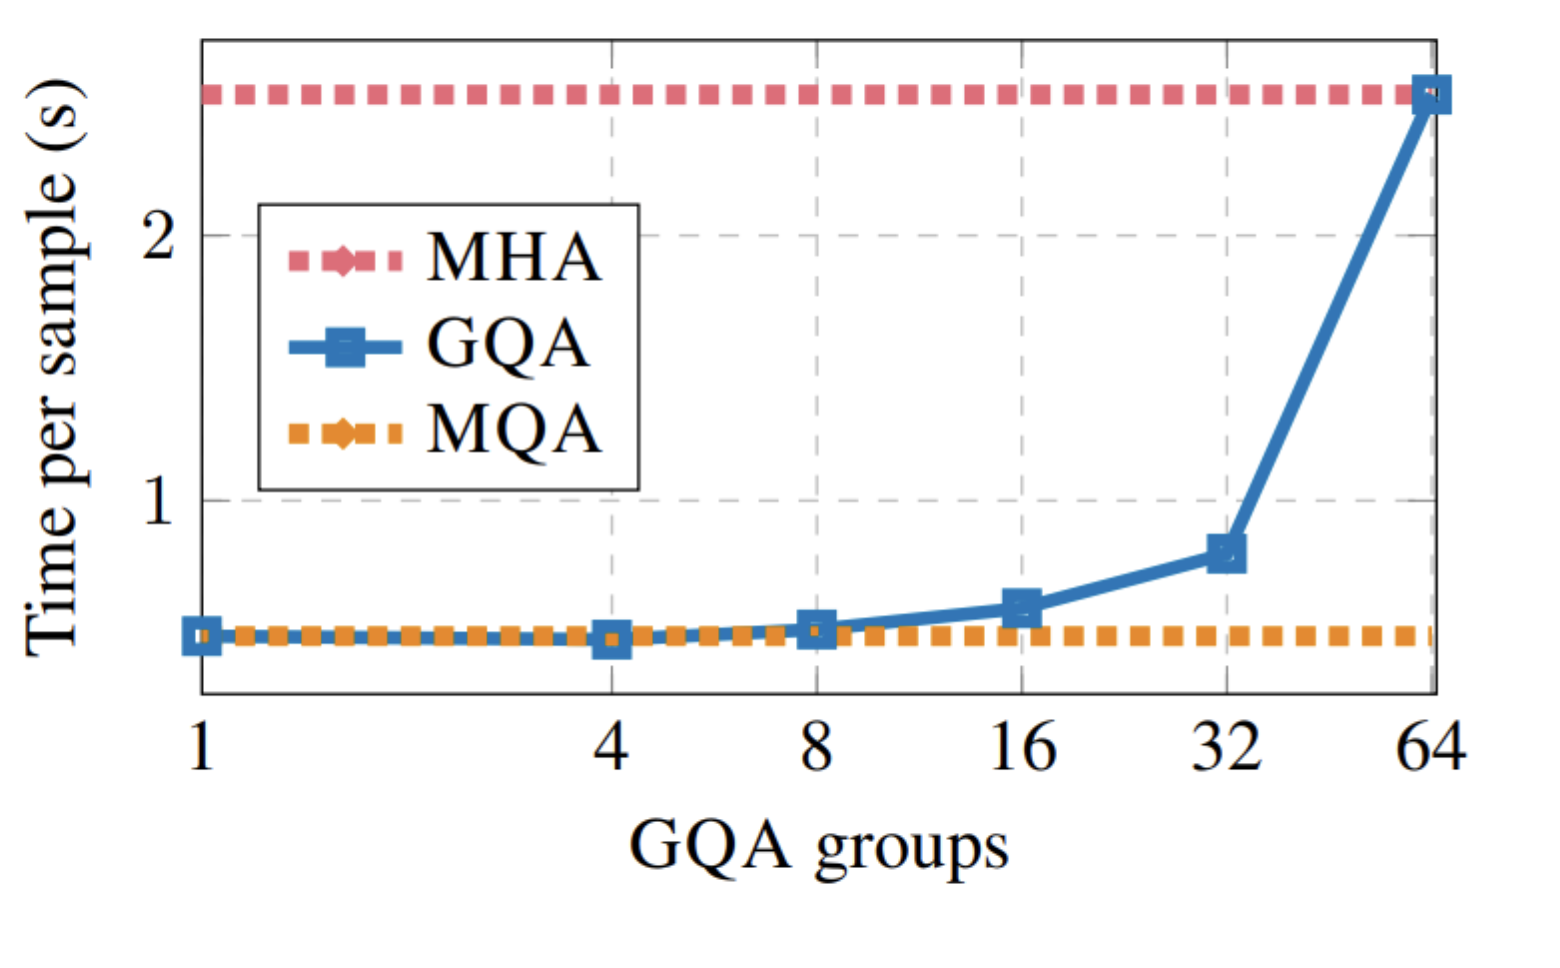
\includegraphics[width=1\linewidth]{graph.png}
\end{figure}

GQA reduces the KV cache by a factor of N / K.

\begin{center}
    Reminder: reducing memory usage leads to speedup (since we're memory-bound).
\end{center}

\begin{minted}{python}
    # Original Llama 2 13B (MHA)
    config = llama2_13b_config({K: 40, B: 64})  
    k40_b64 = compute_transformer_performance_stats(config)  
    
    # GQA with 1:5 ratio (K:N)
    config = llama2_13b_config({K: 8, B: 64})  # Use GQA with 1:5 ratio 
    k8_b64 = compute_transformer_performance_stats(config)  
    Result: Worse latency, but better throughput (and it fits in memory now!)
    
    # Now we can increase the batch size
    config = llama2_13b_config({K: 8, B: 256})  # Increase batch size 
    k8_b256 = compute_transformer_performance_stats(config)  
    Result: Worse latency, but better throughput (and still fits in memory!)
\end{minted}

\subsubsection*{Multi-head latent attention (MLA)}

\begin{itemize}
    \item Normal attention: KV cache consists of K \(=\) W\_K h, V \(=\) W\_V h (N \(*\) H dimensions)
    \item MLA: store compressed vector c \(=\) W\_c h (C dimensions), project up to K \(=\) W\_K c, V \(=\) W\_V c when needed
    \item DeepSeek v2: reduce N \(*\) H \(=\) 16384 to C \(=\) 512
    \item Wrinkle: MLA is not compatible with RoPE, so need to add additional 64 dimensions for RoPE, so 512 \(+\) 64 \(=\) 576 total dimensions
    \item Latency/throughput improvements follow similarly from the KV cache reduction as argued earlier
\end{itemize}

\begin{figure}[hpbt]
    \centering
    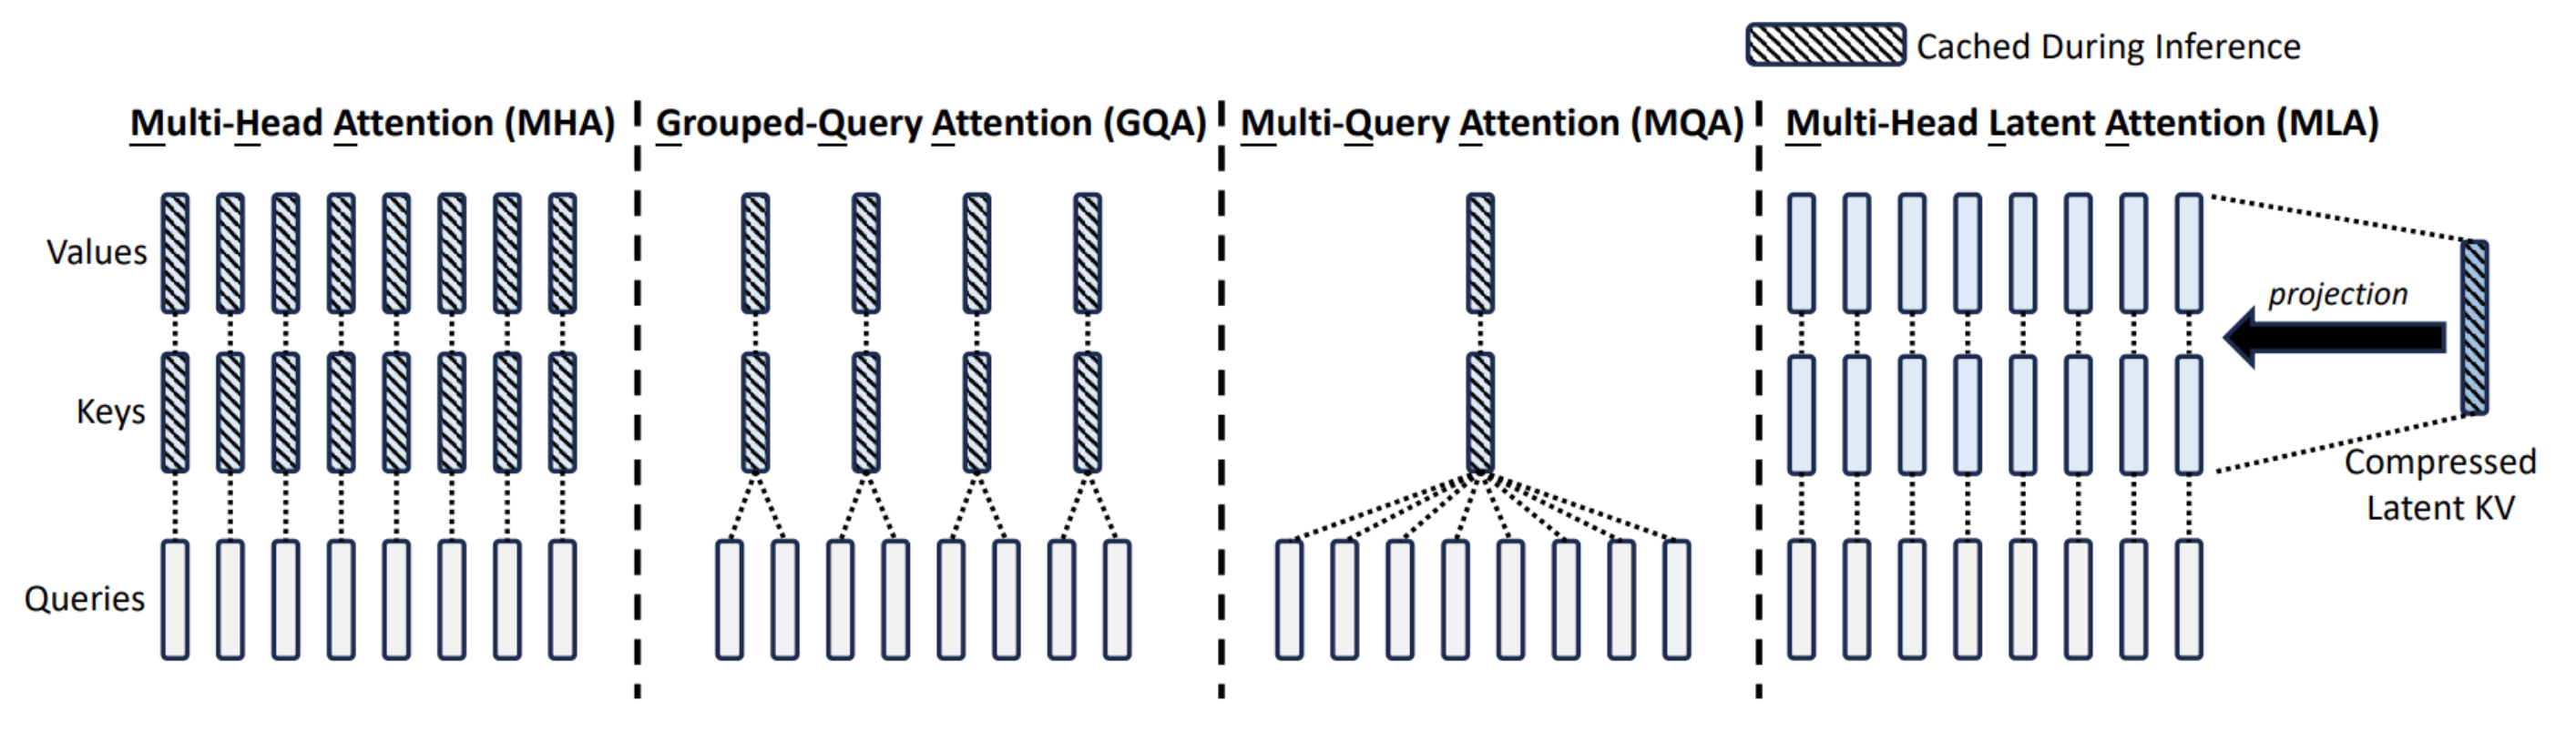
\includegraphics[width=1\linewidth]{mla.png}
\end{figure}

\subsubsection*{Cross-layer attention (CLA)}

Idea: share KVs across layers (just as GQA shares KVs across heads).

\begin{figure}[H]
    \centering
    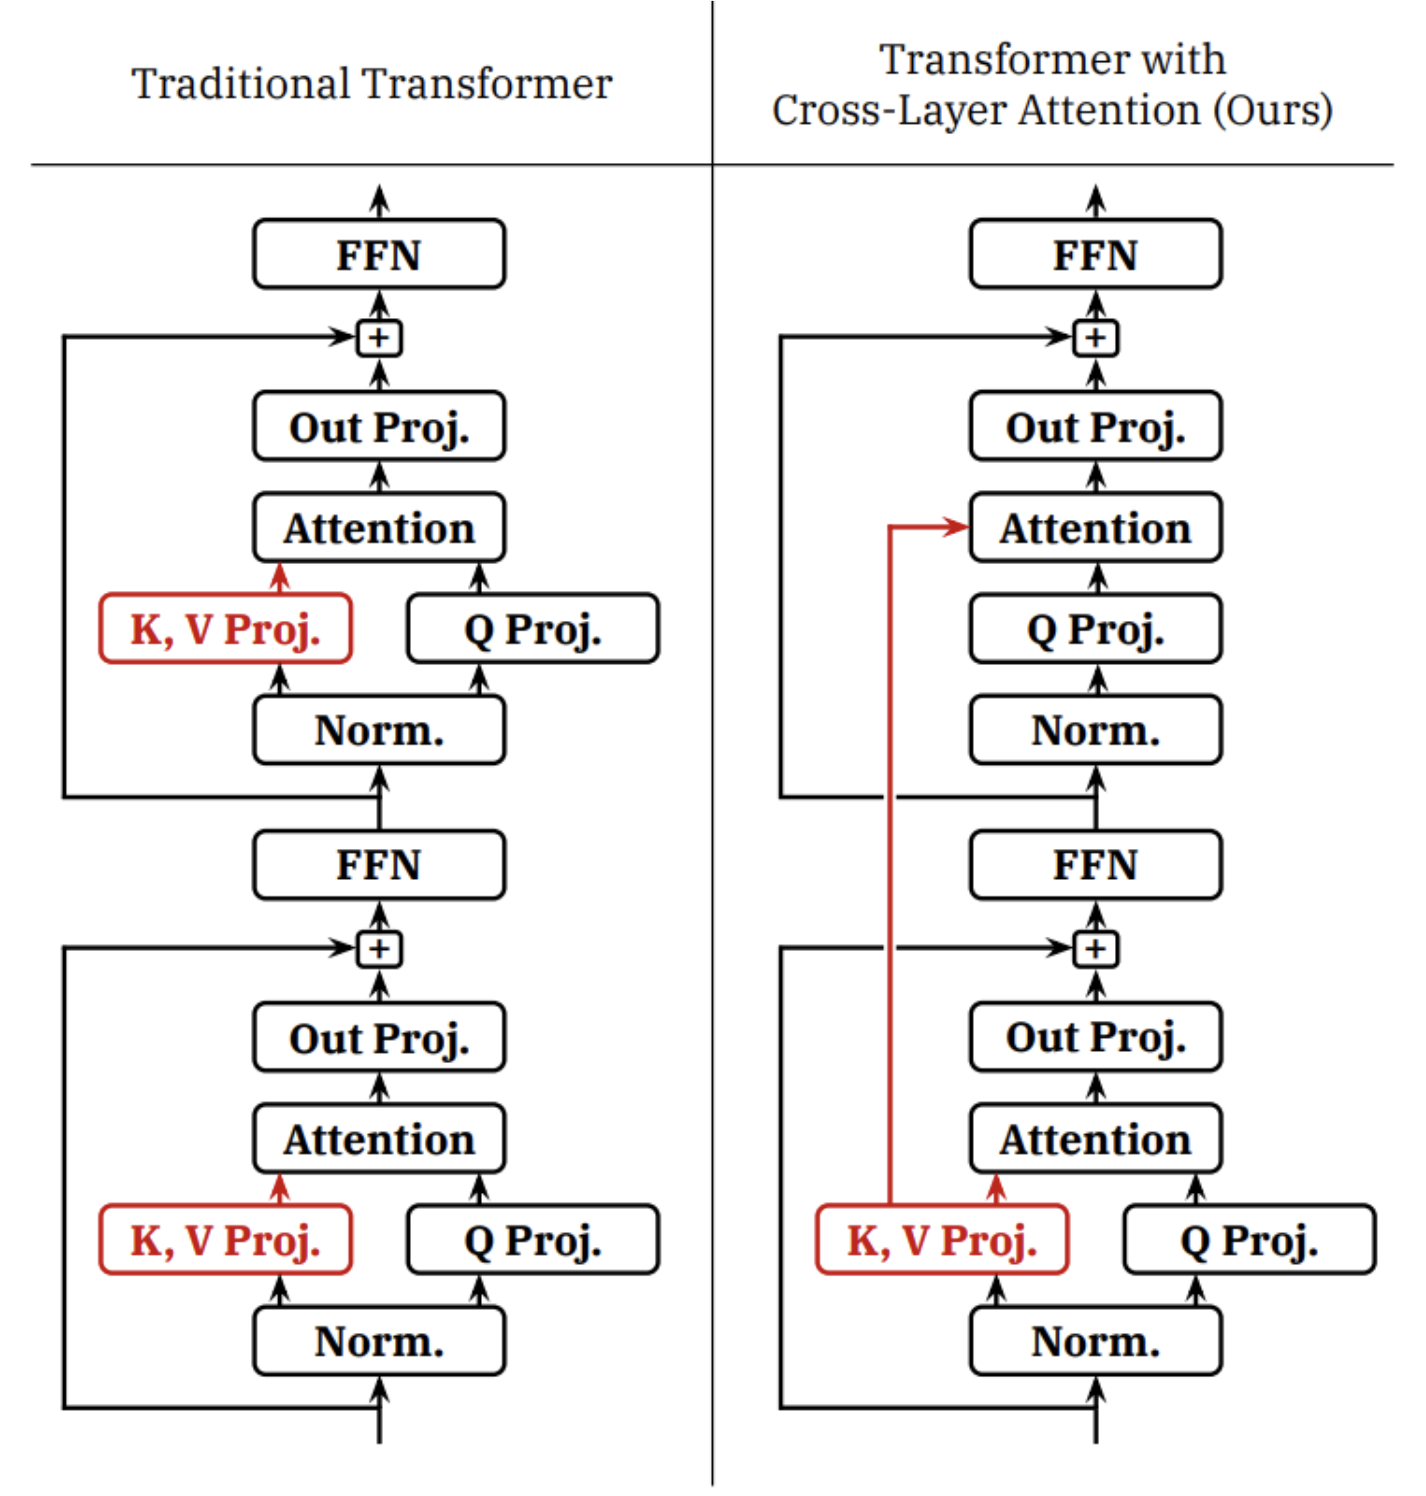
\includegraphics[width=1\linewidth]{CLA.png}
\end{figure}

Empirically improves the pareto frontier of accuracy and KV cache size (latency and throughput).

\subsubsection*{Local (sliding window) attention}

\begin{itemize}
    \item Idea: just look at the local context, which is most relevant for modeling.
    \item Effective context scales linearly with the number of layers.
    \item KV cache is independent of sequence length!
    \item Problem: this can still hurt accuracy.
    \item Solution: interleave local attention with global attention (hybrid layers)!
\end{itemize}

\begin{figure}[hpbt]
    \centering
    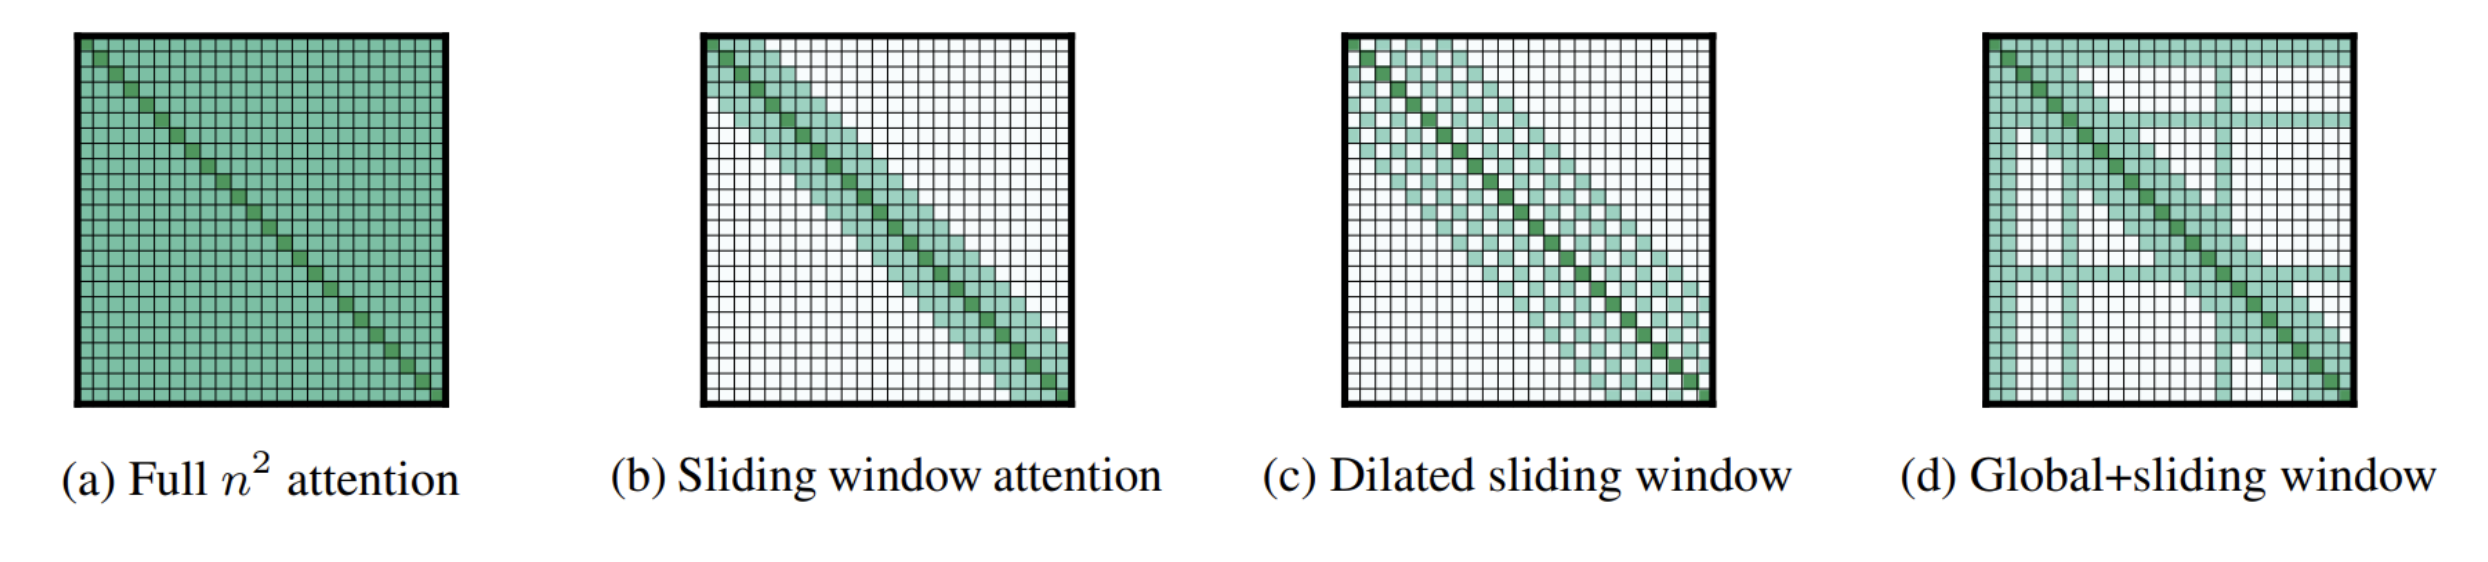
\includegraphics[width=1\linewidth]{sliding_window.png}
\end{figure}

\subsubsection*{DeepSeek v4 attention}

\begin{figure}[hpbt]
    \centering
    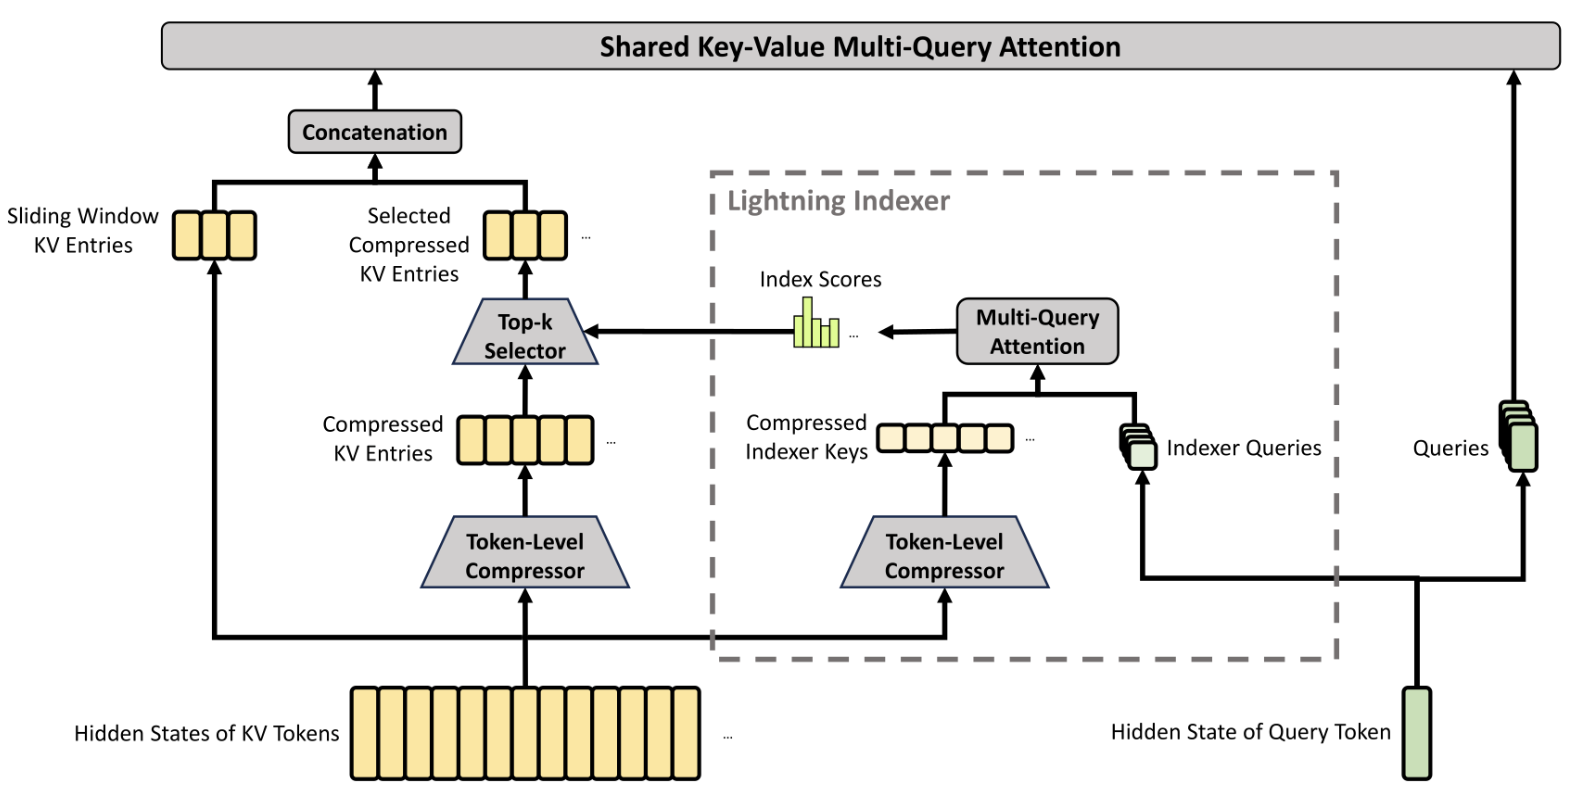
\includegraphics[width=1\linewidth]{dsa.png}
\end{figure}

\begin{itemize}
    \item Supports 1M context length
    \item Compressed Sparse Attention (CSA): compresses every m tokens into 1
    \item DeepSeek Sparse Attention (DSA): selects the top k
    \item Heavily Compressed Attention (HCA): compresses even more
\end{itemize}

Summary:
\begin{itemize}
    \item Goal: reduce the KV cache size (since inference is memory-bound) without hurting accuracy
    \item Lower-dimensional KV cache (GQA, MLA, CLA)
    \item Local attention (truncates the KV cache) on some of the layers
    \item Other ideas: linear attention / state-space-models (Mamba 2, GatedDeltaNet), diffusion models
\end{itemize}

\subsection*{Quantization}

Key idea: reduce the precision of numbers ... less memory means higher latency/throughput (since inference is memory-bound).

\begin{minted}{python}
    # Mechanics
    x = 5.2342  
    scale = 0.1
    zero_point = 4
    x_quant = round(x / scale) + zero_point  # Quantize  
    x_approx = (x_quant - zero_point) * scale  # Dequantize 
\end{minted}

Of course we have to worry about accuracy...

\begin{figure}[hpbt]
    \centering
    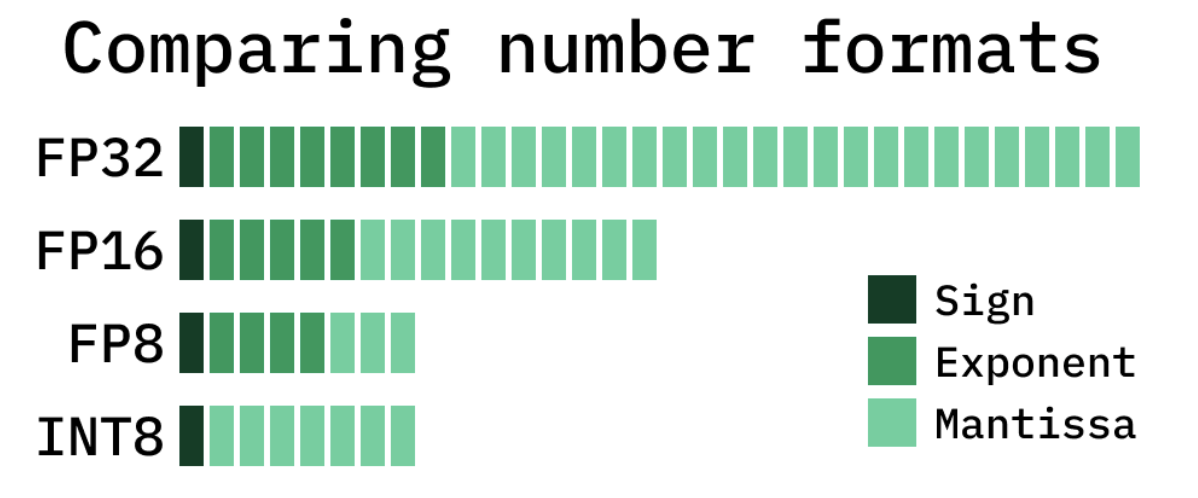
\includegraphics[width=1\linewidth]{quant.png}
\end{figure}

\begin{itemize}
    \item fp32 (4 bytes): needed for parameters and optimizer states during training
    \item bf16 (2 bytes): default for inference
    \item fp8 (1 byte) [-240, 240] for e4m3 on H100s: can train if you dare
    \item int8 (1 byte) [-128, 127]: less accurate but cheaper than fp8, but for inference only
    \item int4 (0.5 bytes) [-8, 7]: cheaper, even less accurate
\end{itemize}

Quantization-aware training (QAT)
\begin{itemize}
    \item During training, quantize-and-dequantize during the forward pass to simulate quantization errors
    \item Pro: weights are trained to work with quantization
    \item Con: requires expensive large-scale training
\end{itemize}

Post-training quantization (PTQ):
\begin{itemize}
    \item Done after training, so much cheaper
    \item Run on sample data to determine scale and zero point for each layer or tensor
    \item GPTQ: use Hessian information to update non-quantized weights to account for quantization error
\end{itemize}

\subsubsection*{Activation-aware quantization (AWQ)}

\begin{figure}[hpbt]
    \centering
    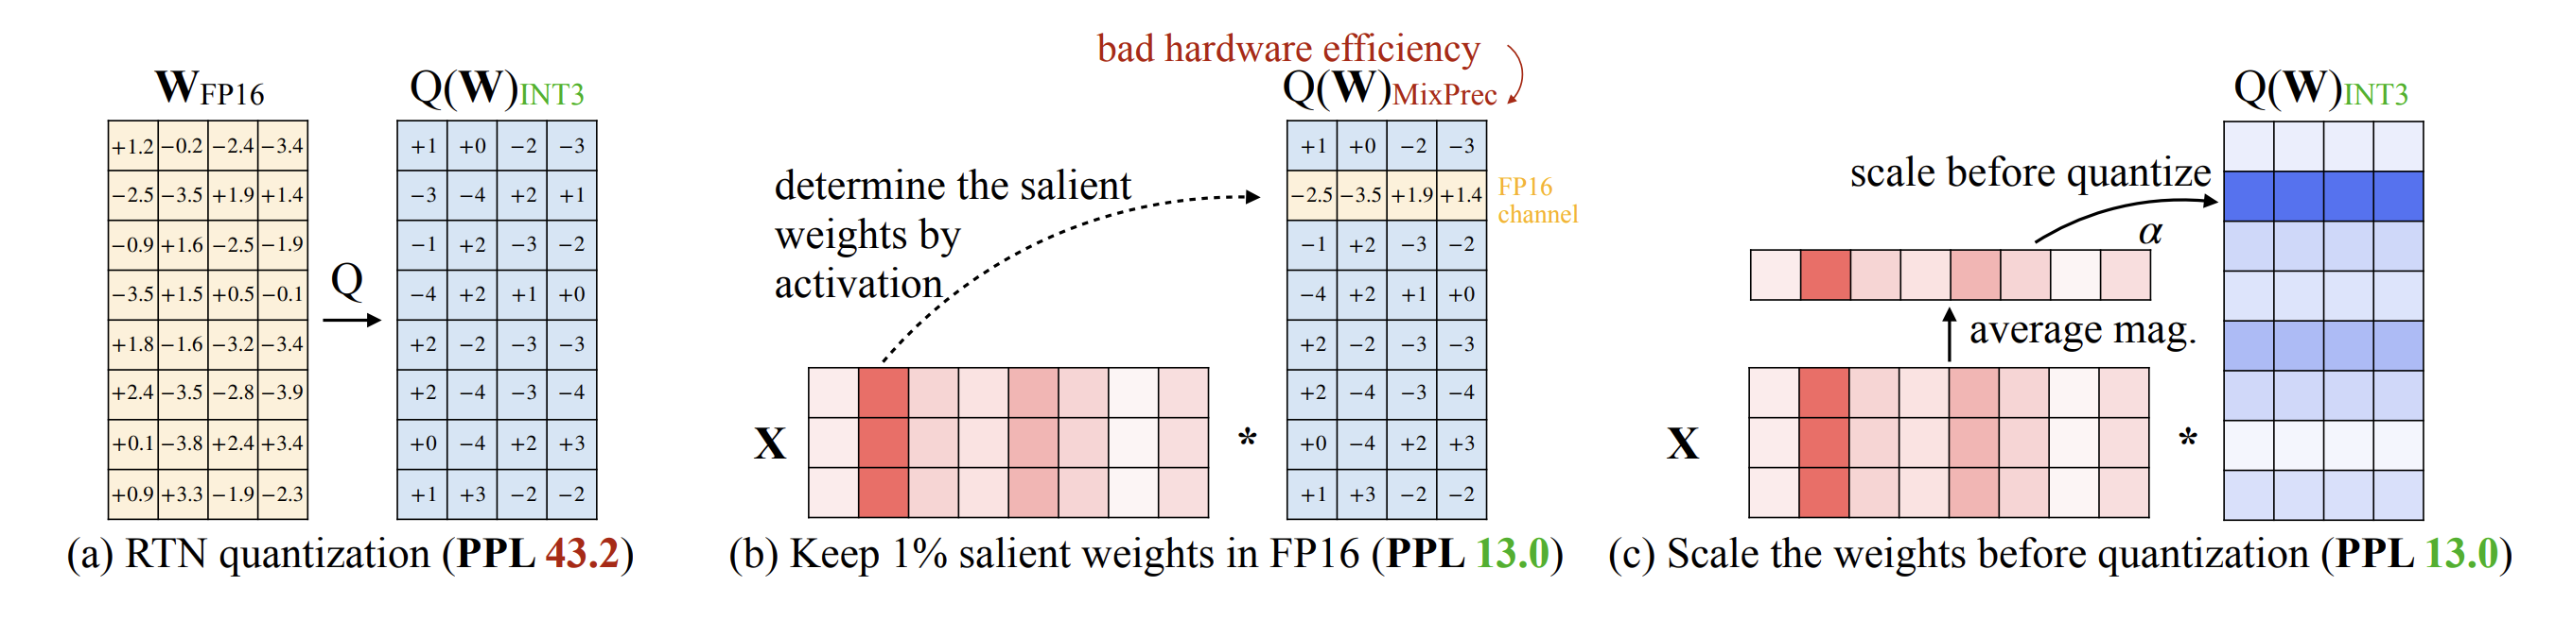
\includegraphics[width=1\linewidth]{AWQ.png}
\end{figure}

\begin{itemize}
    \item Observation: some activation channels are large
    \item Weights that hit those matter more
    \item Allocate more precision to those weights
    \item Idea: select which weights (0.1-1\%) to keep in high precision based on activations
    \item fp16 \(\to\) int3 produces 4\(\times\) lower memory, 3.2\(\times\) speedup
\end{itemize}

\subsection*{Model pruning}

Key idea: just rip out parts of an expensive model to make it cheaper ...and then fix it up.

\begin{figure}[hpbt]
    \centering
    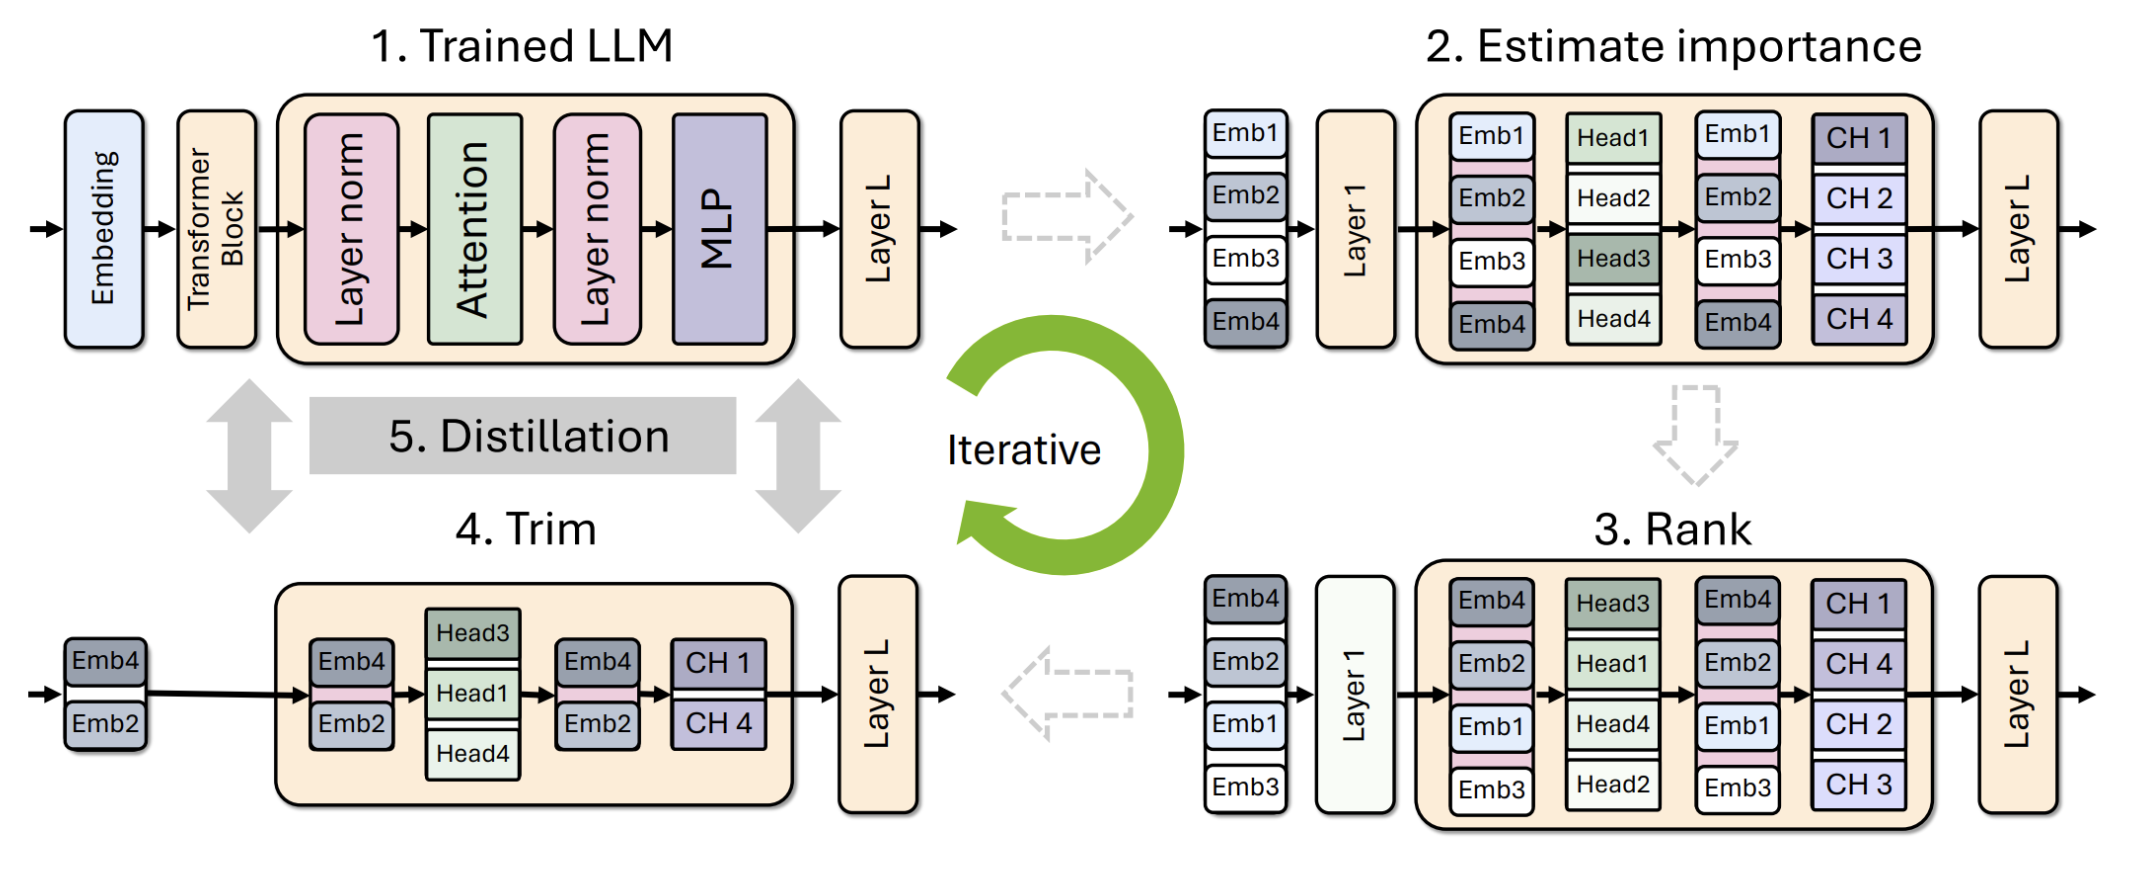
\includegraphics[width=1\linewidth]{pruning.png}
\end{figure}

Algorithm:
\begin{enumerate}
    \item Identify important {layer, head, hidden dimension} on a small calibration dataset
    \item Remove unimportant layers to get a smaller model
    \item Distill the original model into pruned model
\end{enumerate}

\begin{figure}[hpbt]
    \centering
    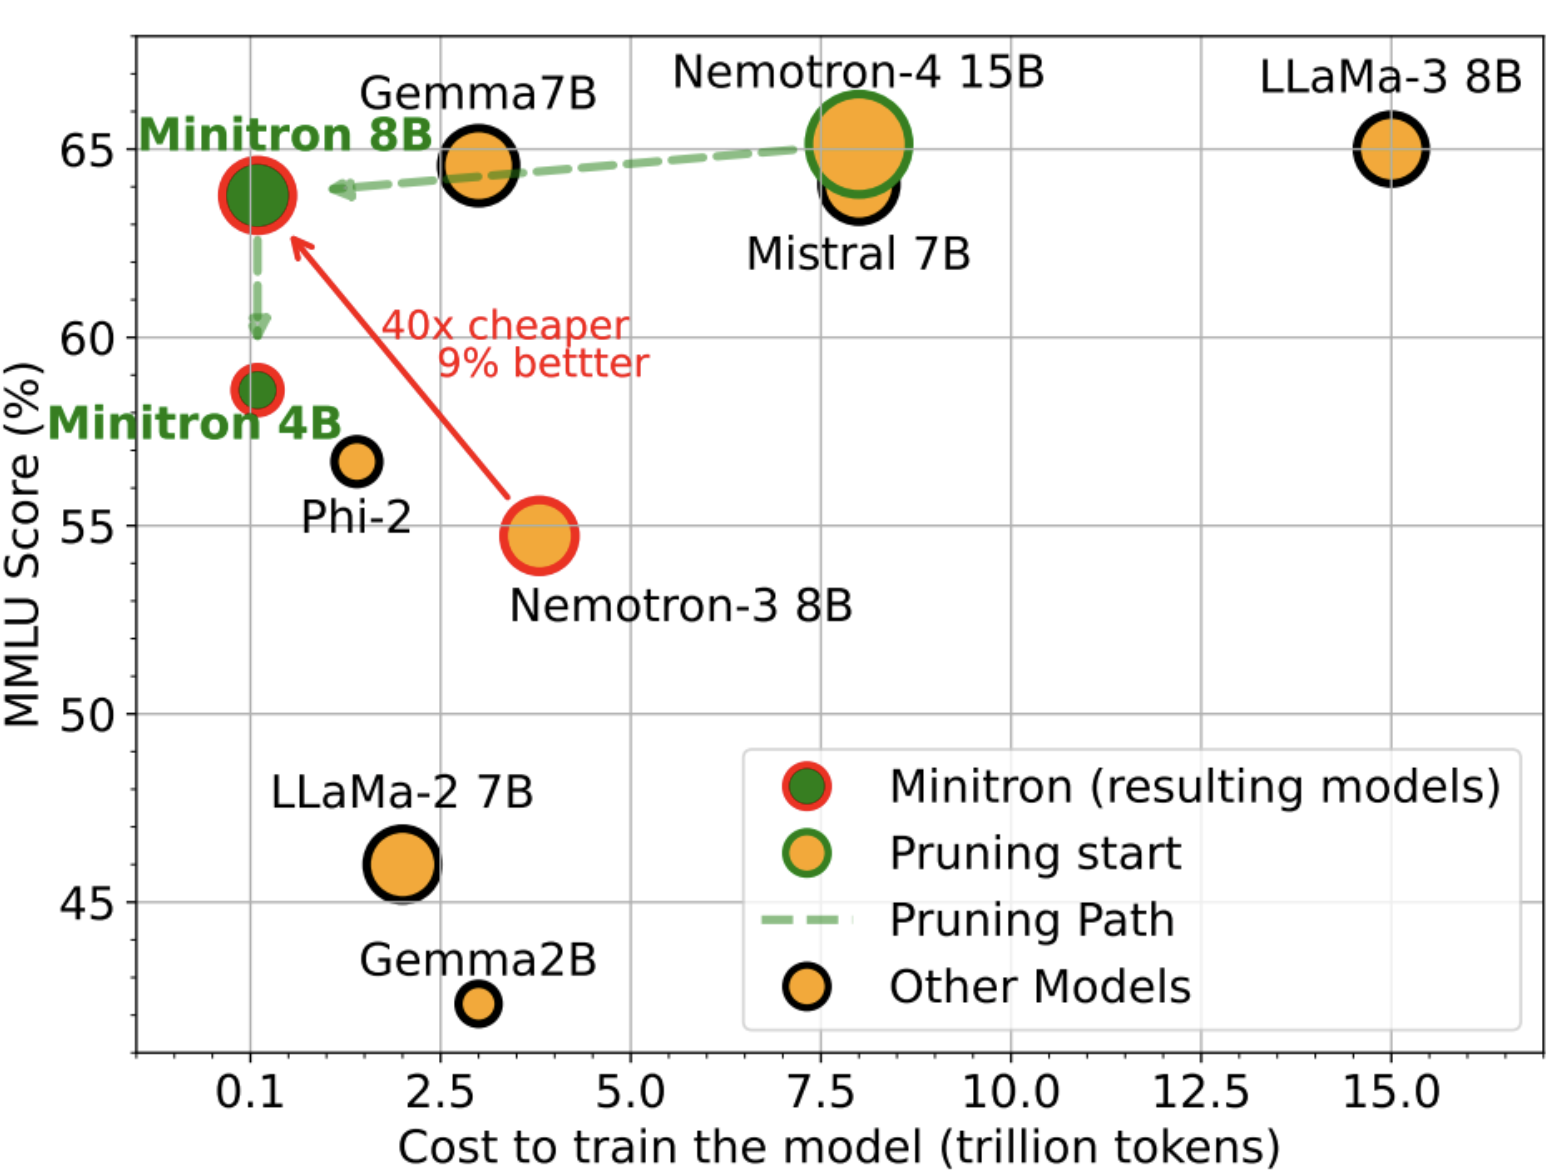
\includegraphics[width=0.66\linewidth]{NVIDIA.png}
\end{figure}

\subsection*{Speculative decoding}

Recall the two stages of inference:
\begin{itemize}
    \item Prefill: given a sequence, encode tokens in parallel (compute-bound) [note: also gives you probabilities]
    \item Generation: generate one token at a time (memory-bound)
\end{itemize}

In other words, checking is faster than generation. \\

Speculative sampling 
\begin{itemize}
    \item Use a cheaper draft model p to guess a few tokens (e.g., 4)
    \item Evaluate with target model q (process tokens in parallel), and accept if it looks good
\end{itemize}

\begin{figure}[hpbt]
    \centering
    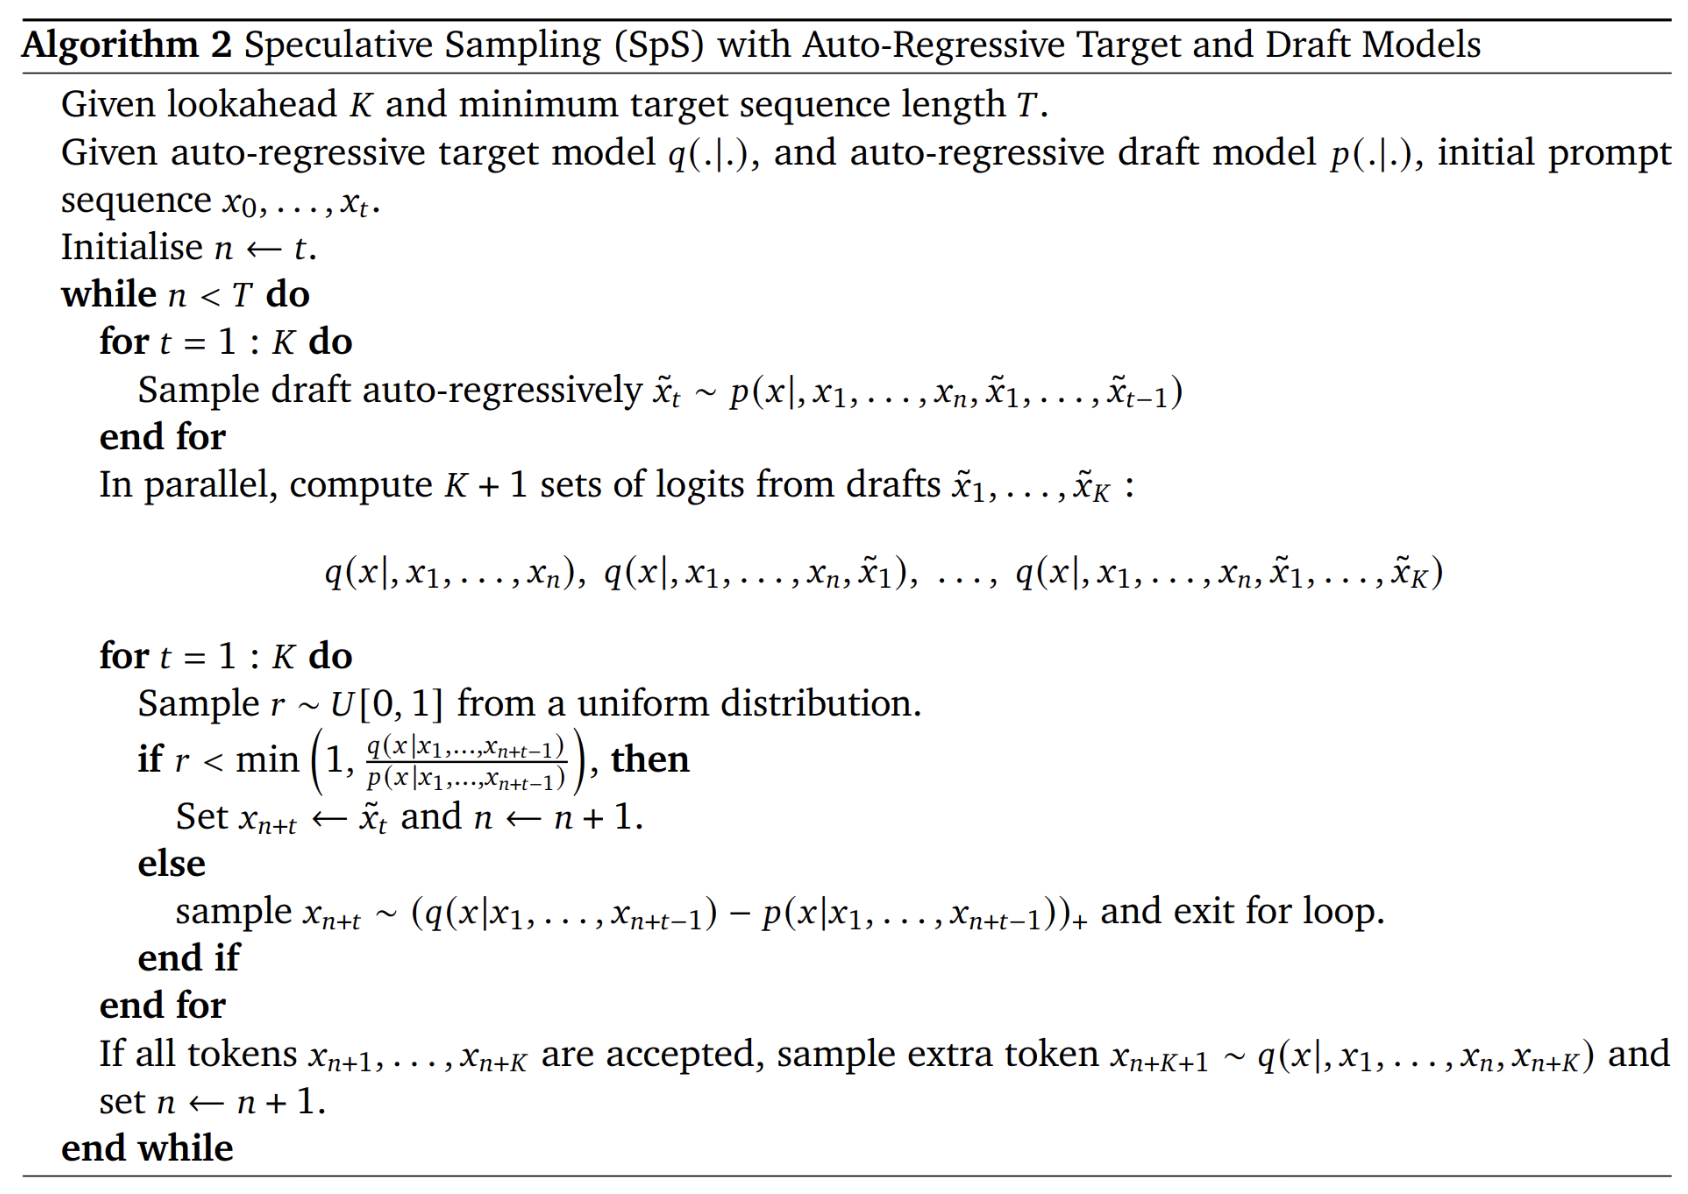
\includegraphics[width=1\linewidth]{algorithm.png}
\end{figure}

This is modified rejection sampling with proposal p and target q.

\begin{itemize}
    \item Modification: always generate at least one candidate (rejection sampling will keep looping)!
    \item Key property: guaranteed to be an \textbf{exact sample} from the target model!
\end{itemize}

Proof by example: assume two vocabulary elements \(\{A, B\}\)

\begin{itemize}
    \item Draft model probabilities: [p(A), p(B)].
    \item Target model probabilities: [q(A), q(B)].
    \item Assume p(A) \(>\) q(A) [draft model oversamples A].
    \item Therefore p(B) \(<\) q(B) [draft model undersamples B].
    \item Residual probabilities \(max(q-p, 0)\): \([0, 1]\).
\end{itemize}

Compute the probabilities of speculatively sampling a token:

\begin{itemize}
    \item P[sampling A] \(=\) p(A) \(*\) (q(A) / p(A)) \(+\) p(B) \(*\) 1 \(*\) 0 = q(A)
    \item P[sampling B] \(=\) p(B) \(*\) 1 \(+\) p(A) \(*\) (1 \(-\) q(A) \(/\) p(A)) \(*\) 1 = q(B)
\end{itemize}

In practice:
\begin{itemize}
    \item Target model has 70B parameters, draft model has 8B parameters
    \item Target model has 8B parameters, draft model has 1B parameters
    \item Try to make draft model as close to target (distillation)
\end{itemize}

Extensions to improve the draft model:
\begin{itemize}
    \item Medusa: draft model generates multiple tokens in parallel
    \item EAGLE: draft model takes high-level features from target model
\end{itemize}

\begin{figure}[hpbt]
    \centering
    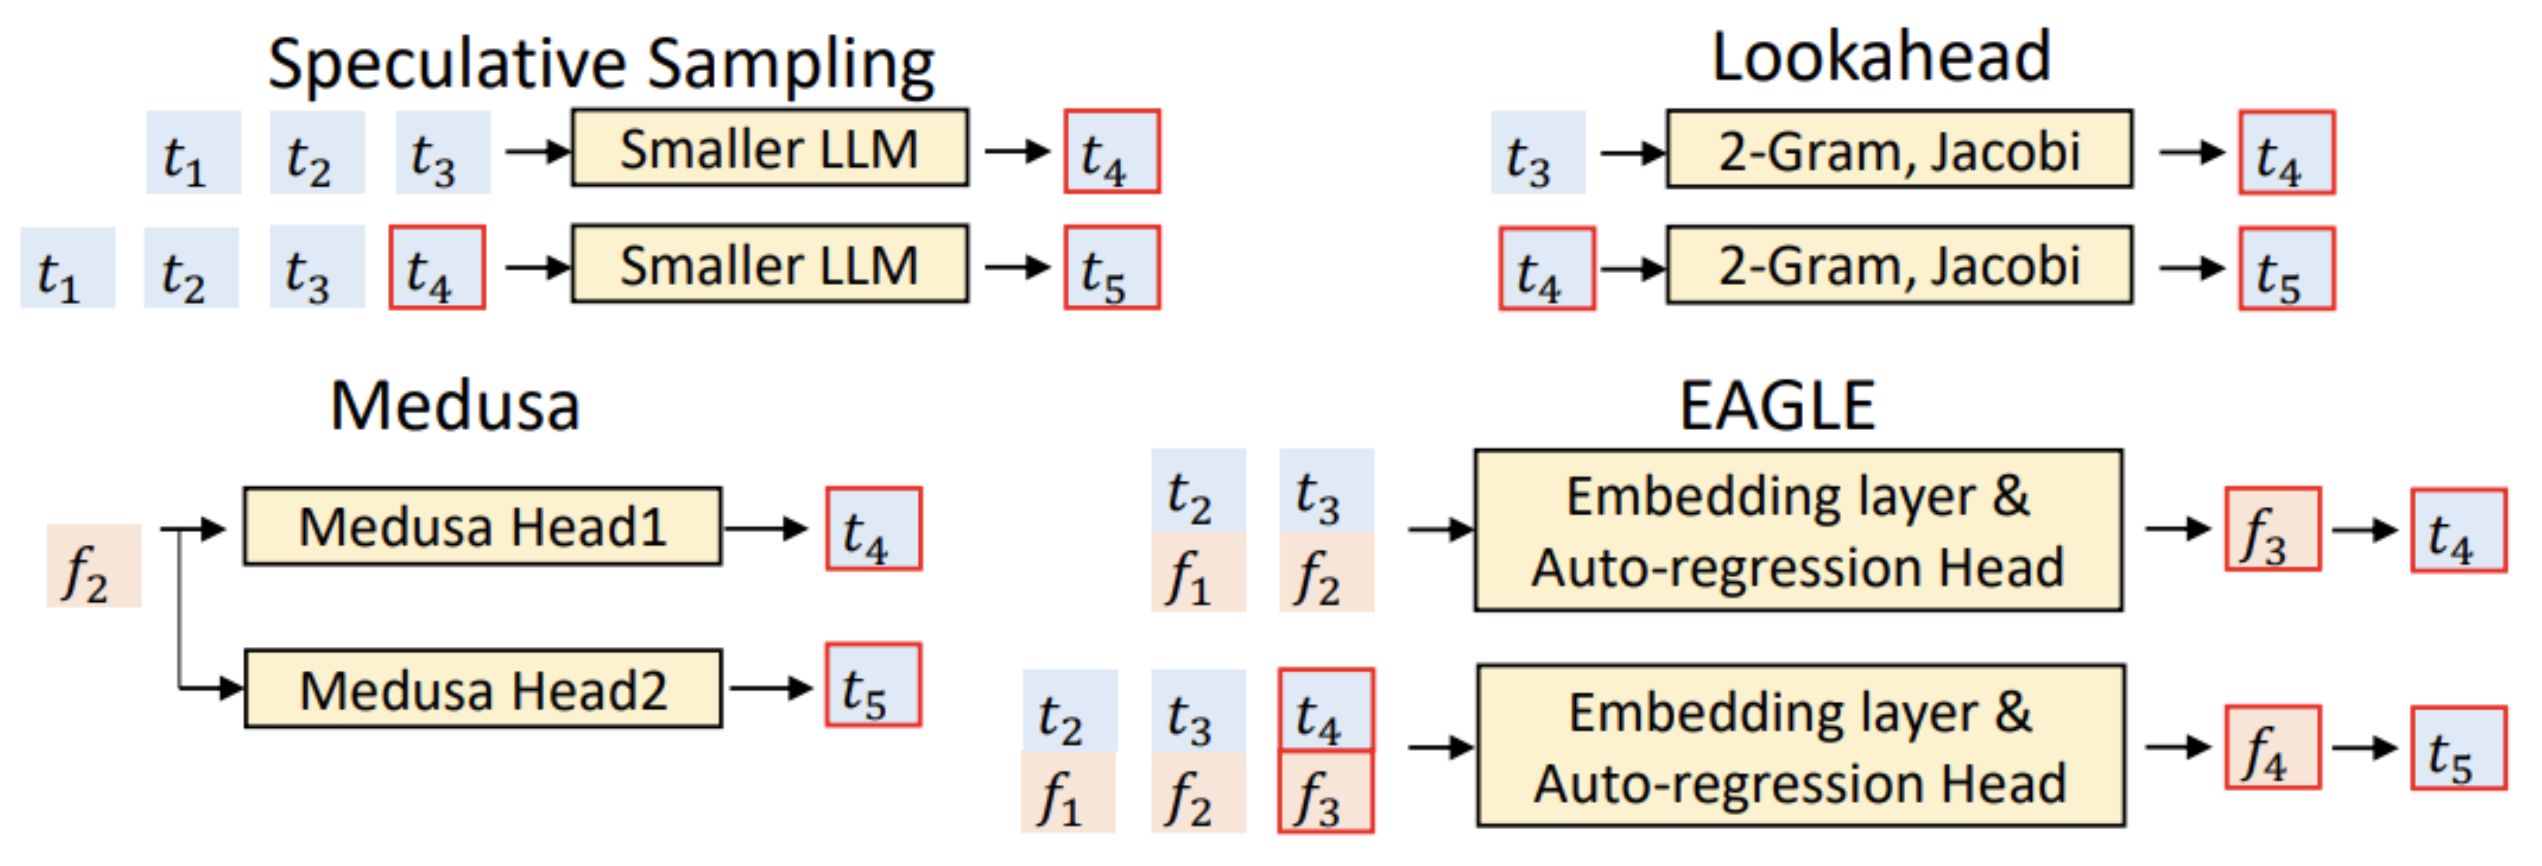
\includegraphics[width=1\linewidth]{spec.png}
\end{figure}

Summary:
\begin{itemize}
    \item Exact sampling from target model (thanks to math)!
    \item Exploits asymmetry between checking and generation
    \item Lots of room for innovation on the draft model (involves training)
\end{itemize}

\subsection*{Continuous batching}

\begin{figure}[hpbt]
    \centering
    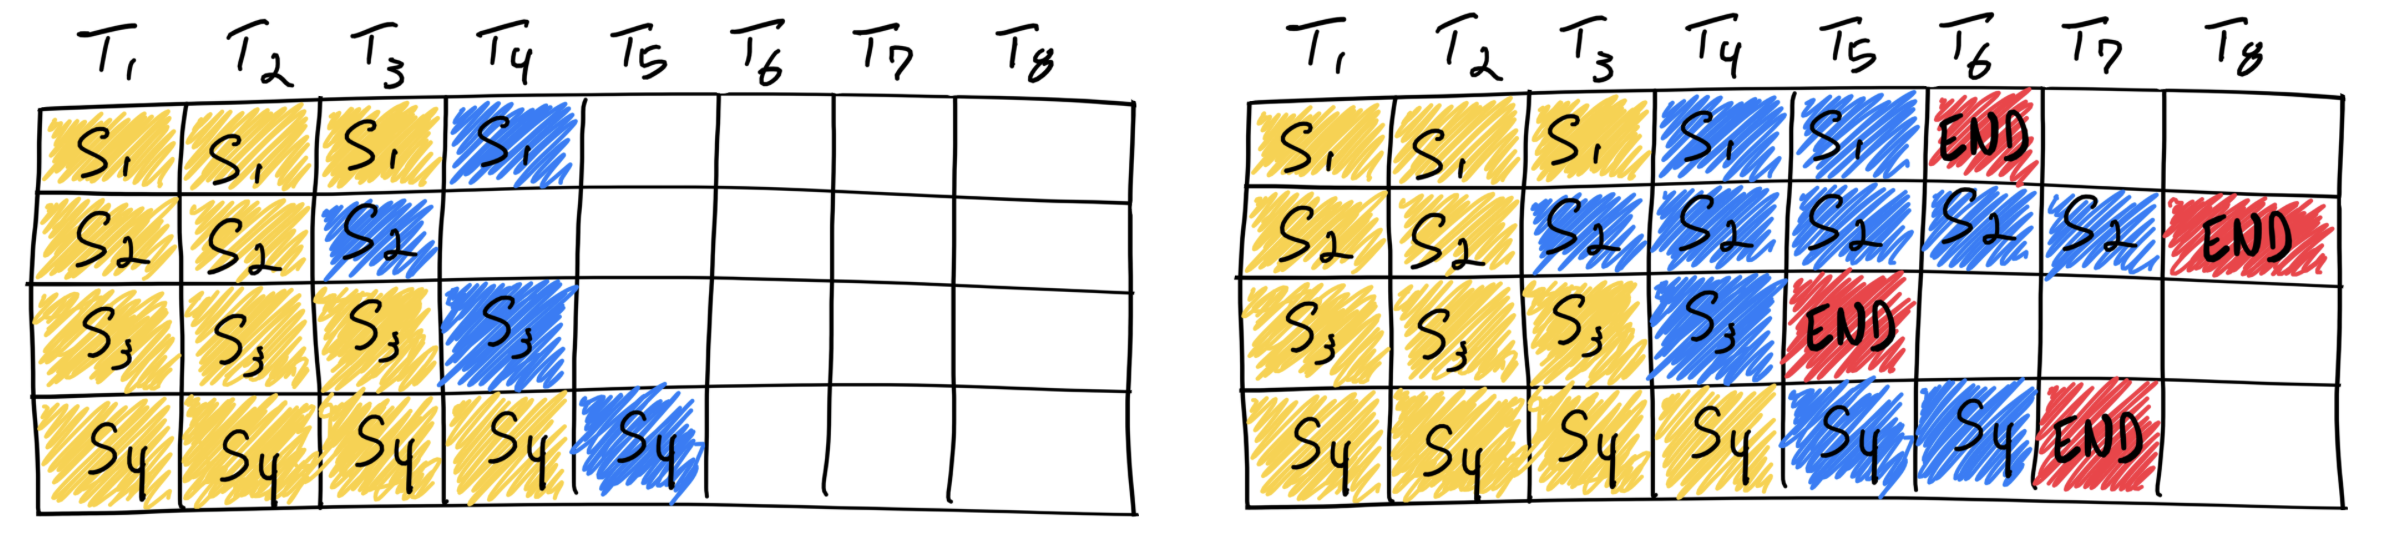
\includegraphics[width=1\linewidth]{batching.png}
\end{figure}

Problem:
\begin{itemize}
    \item Training: get a dense block of tokens (batch size x sequence length)
    \item Inference: requests arrive and finish at different times, so you have a ragged array
\end{itemize}

Solution: iteration-level scheduling
\begin{itemize}
    \item Decode step by step
    \item Add new requests to the batch as they arrive (so don't have to wait until generation completes)
\end{itemize}

Problem: 
\begin{itemize}
    \item Batching only works when all sequences have the same dimensionality (right?)
    \item But each request might have a different length
\end{itemize}

Solution: selective batching
\begin{itemize}
    \item Training: when all sequences of the same length, operate on a B \(\times\) S \(\times\) H tensor
    \item But we might have different lengths: [3, H], [9, H], [5, H], etc.
    \item Attention computation: process each sequence separately
    \item Non-attention computation: concatenate all the sequences together to [3 \(+\) 9 \(+\) 5, H]
\end{itemize}

\subsection*{Paged attention}

Previous status quo:
\begin{itemize}
    \item Request comes in
    \item Allocate section of KV cache for prompt and response (up to a max length)
\end{itemize}

\begin{figure}[hpbt]
    \centering
    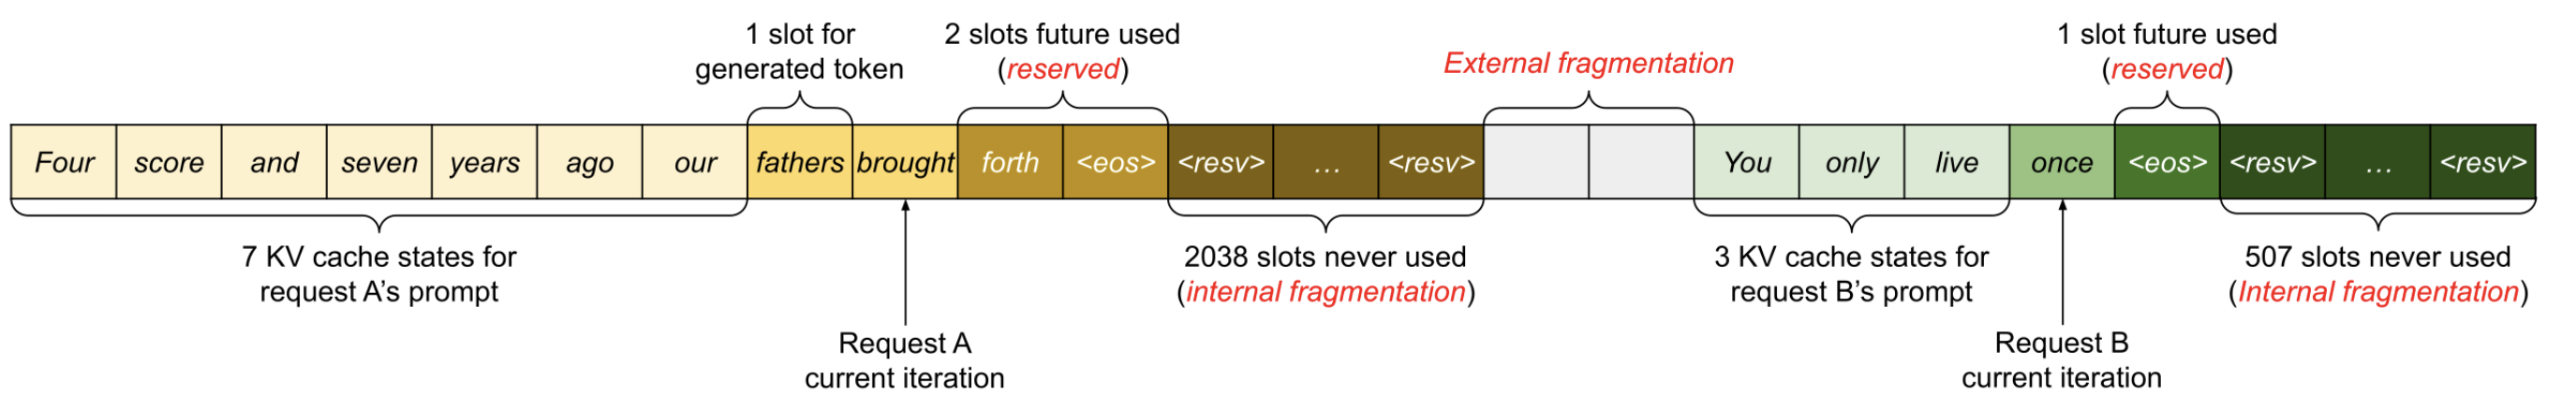
\includegraphics[width=1\linewidth]{OS.png}
\end{figure}

Problem: fragmentation (what happens to your hard drive)
\begin{itemize}
    \item But this is wasteful since we might generate much fewer tokens (internal fragmentation)!
    \item Might be extra unused space between sections (external fragmentation)!
\end{itemize}

Solution: PagedAttention (remember operating systems)
\begin{itemize}
    \item Divide the KV cache of a sequence into non-contiguous \textbf{blocks}
    \begin{figure}[hpbt]
        \centering
        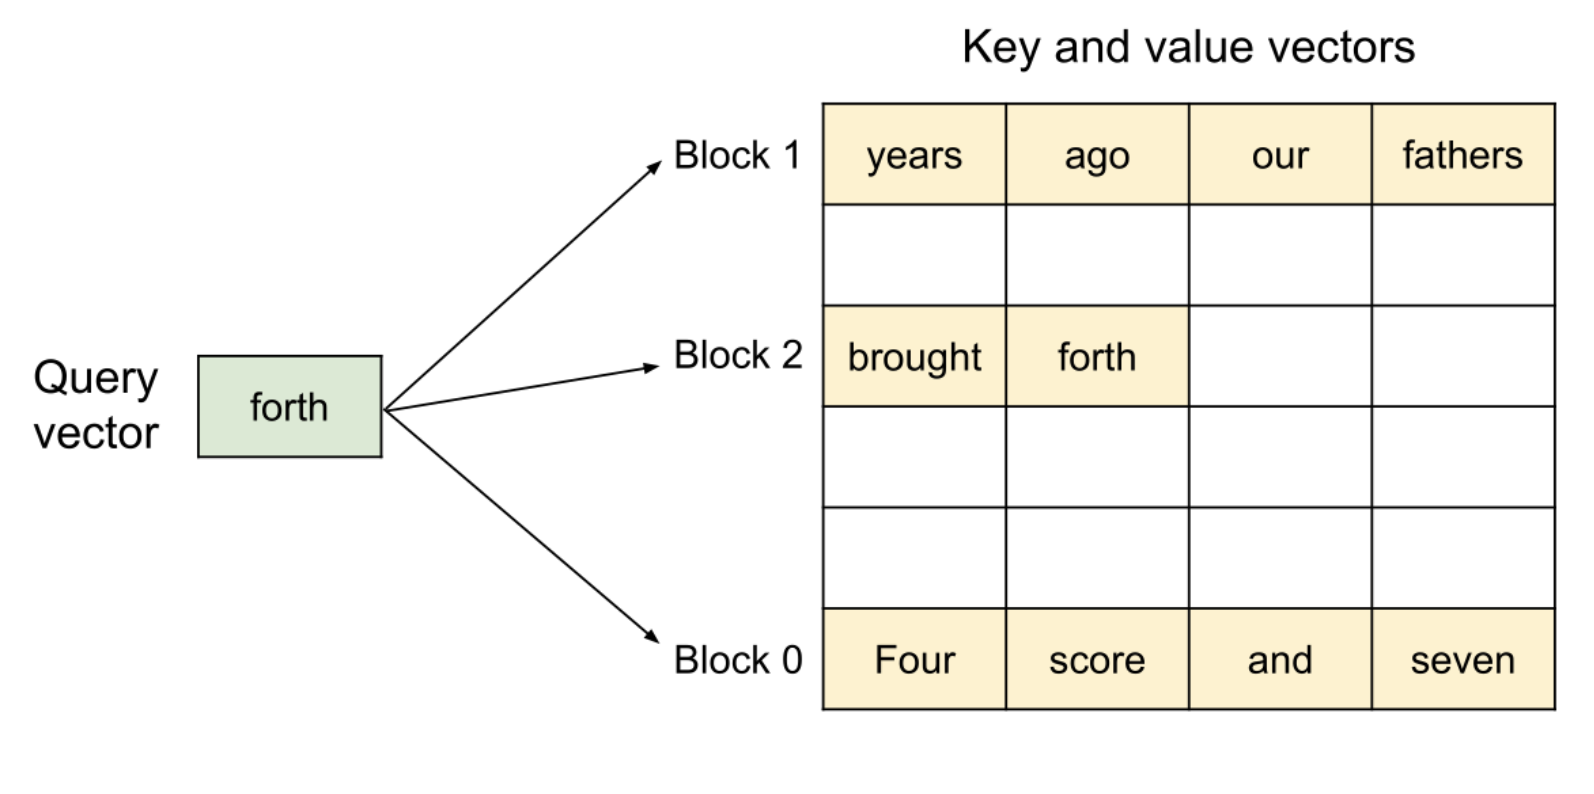
\includegraphics[width=1\linewidth]{partition.png}
    \end{figure}
    \item Two requests share the KV caches 
\end{itemize}

In general, multiple types of sharing KV caches across sequences:

\begin{itemize}
    \item Sharing the system prompt
    \item Sampling multiple responses per prompt (e.g., for program synthesis)
\end{itemize}

Solution: share prefixes, copy-on-write at the block level.

\begin{figure}[H]
    \centering
    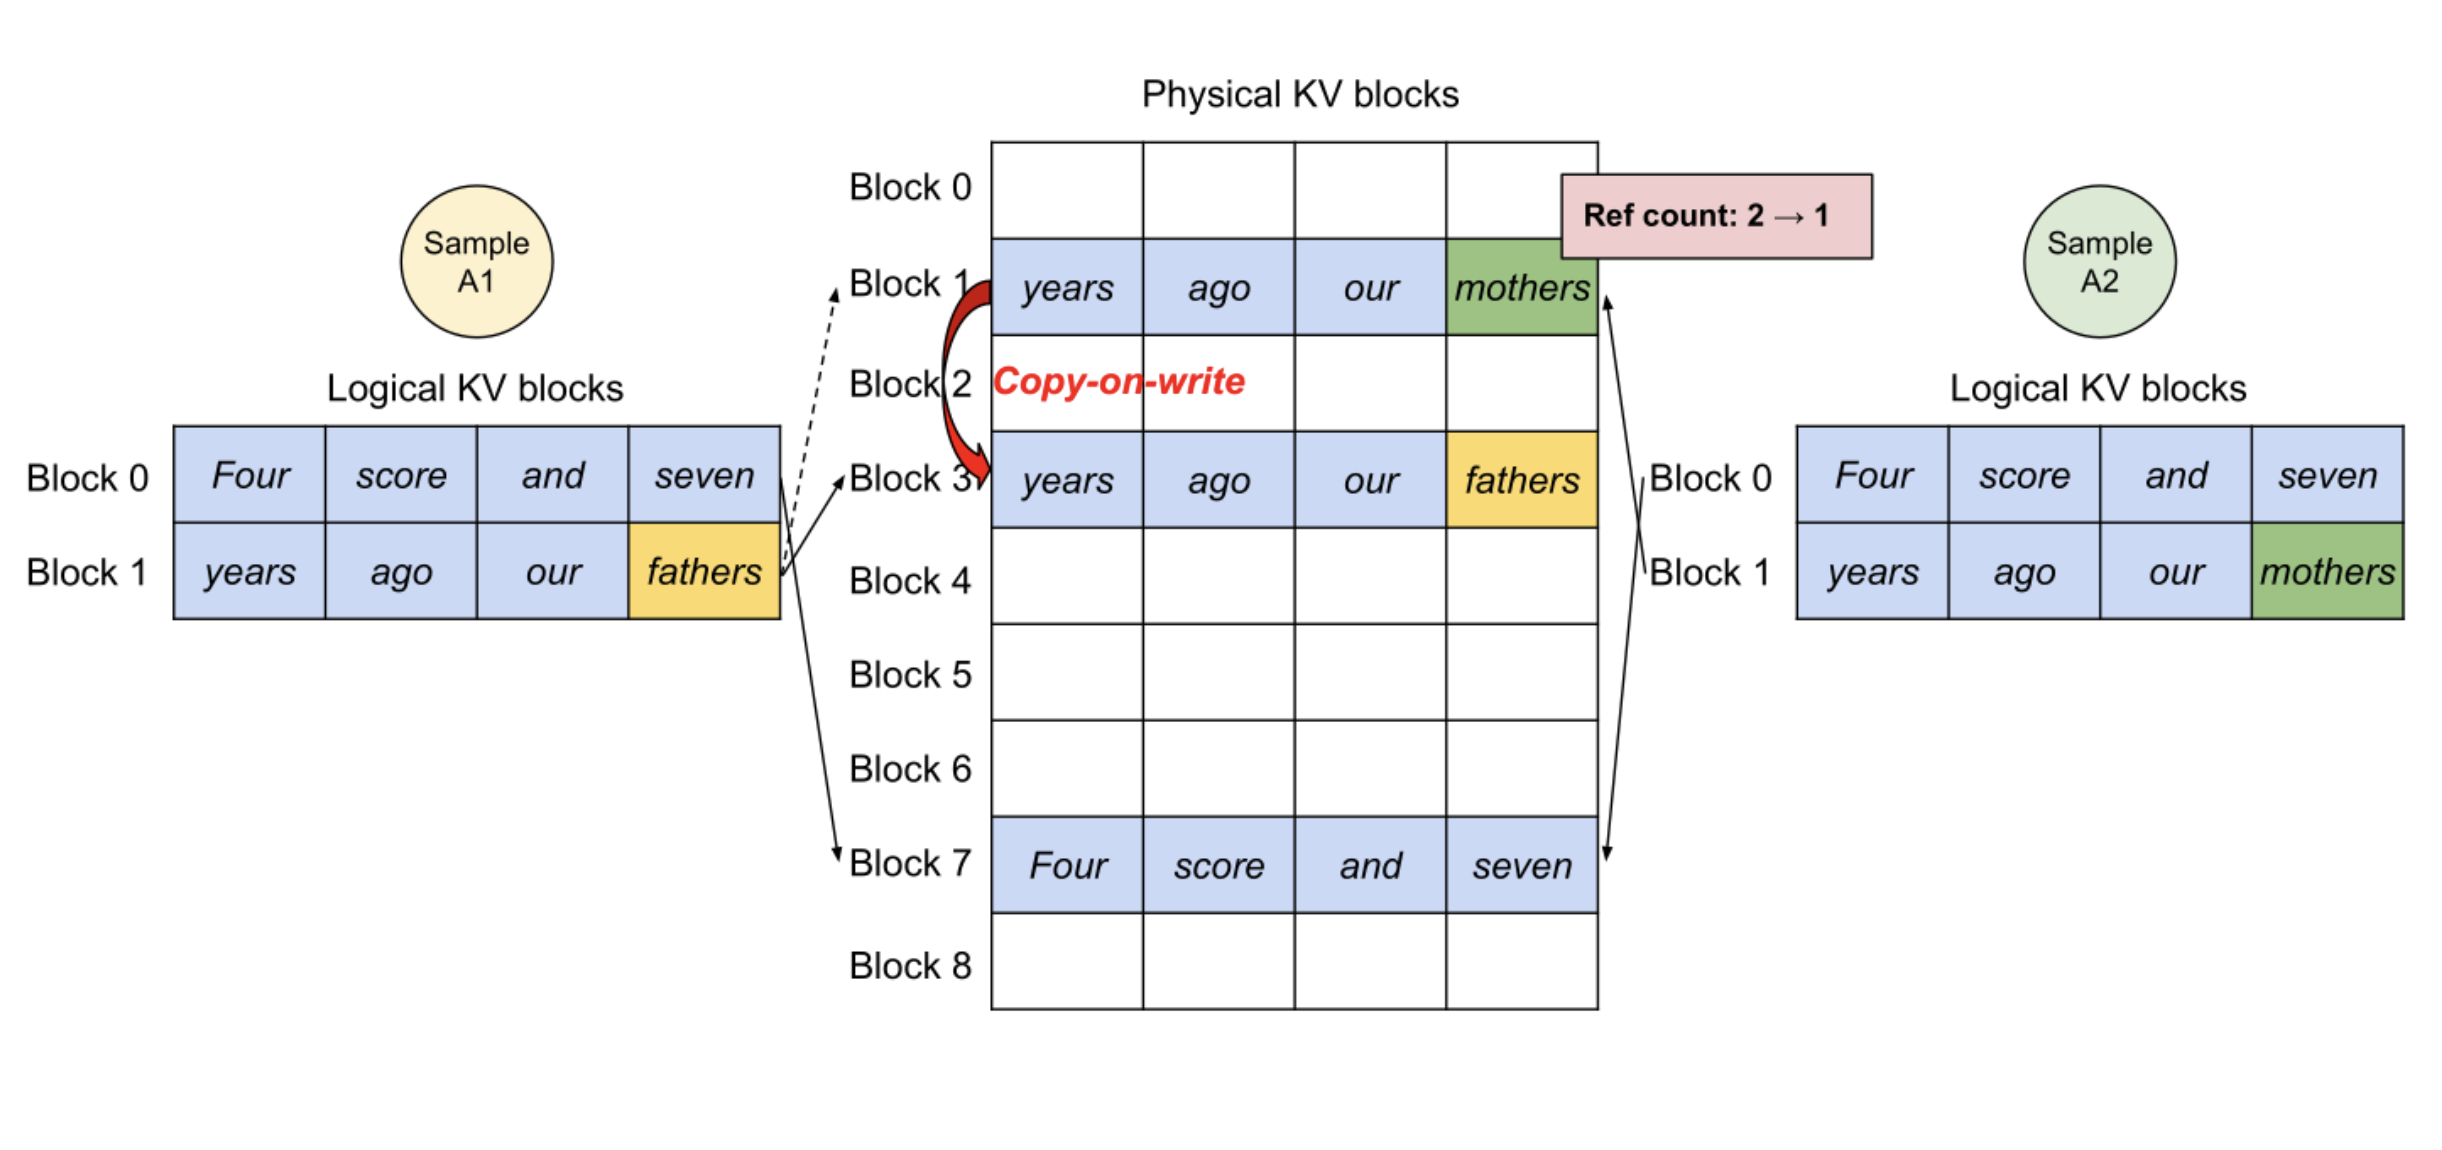
\includegraphics[width=1\linewidth]{paged.png}
\end{figure}

Other vLLM optimizations:

\begin{itemize}
    \item Kernel to fuse block read and attention (reduce kernel launch overhead)
    \item Use latest kernels (FlashAttention, FlashDecoding)
    \item Use CUDA graphs to avoid kernel launch overhead
\end{itemize}

Summary: use ideas from operating systems (paging) to make use of memory for dynamic workloads.

\end{document}
